\section{Funciones Lipschitzianas}

\subsection{Introducción a las funciones Lipschitzianas}
En el estudio introductorio de las ecuaciones diferenciales, el enfoque principal radica en la obtención de soluciones explícitas y el análisis de sus propiedades básicas. Sin embargo, dado que la mayoría de los problemas no admiten una solución analítica cerrada, resulta indispensable adoptar una perspectiva cualitativa para estudiar la existencia, unicidad y el comportamiento de las soluciones.

En este contexto, el concepto de \textbf{función Lipschitziana} desempeña un papel central. Como se demostrará mediante el Teorema de Cauchy-Lipschitz, la mera continuidad de una función no es suficiente para garantizar la \textbf{unicidad de la solución} de un problema de valor inicial. La condición de Lipschitz proporciona la regularidad necesaria para asegurar dicha unicidad. Asimismo, la distinción entre funciones global y localmente Lipschitzianas es determinante para establecer si una solución está definida globalmente en el tiempo o si, por el contrario, deja de existir en un tiempo finito (fenómeno comúnmente denominado ``explosión'' o \textit{blow-up}), aspecto que se detallará al abordar el estudio de las soluciones maximales.

\begin{definición}[Función Globalmente Lipschitziana]
    Sea $\Omega \subset \mathbb{R}^n$ un conjunto abierto y sea $F : \Omega \to \mathbb{R}^n$ una función continua. Se dice que $F$ es \textbf{globalmente Lipschitziana en $\Omega$} si existe una constante $L > 0$ tal que
    \[
        \| F(u) - F(v) \| \leq L \| u - v \| \quad \forall u, v \in \Omega
    \]
    En espacios de dimensión finita, como $\mathbb{R}^n$, la elección de la norma es irrelevante para la validez de esta propiedad, dado que todas las normas son equivalentes. La constante $L$ recibe el nombre de \textbf{constante de Lipschitz} de la función $F$.
\end{definición}

En la práctica, numerosas funciones de interés físico y matemático no satisfacen esta condición en todo el espacio (por ejemplo, los polinomios de grado estrictamente mayor que uno). No obstante, es frecuente que presenten un comportamiento lo suficientemente regular si se restringe su dominio a regiones acotadas.

\begin{definición}[Función Localmente Lipschitziana]
    Sea $\Omega \subset \mathbb{R}^n$ un conjunto abierto y sea $F : \Omega \to \mathbb{R}^n$ una función continua. Se dice que $F$ es \textbf{localmente Lipschitziana en $\Omega$} cuando para todo $u_0 \in \Omega$ existe un radio $R > 0$ tal que la bola abierta $B(u_0, R)$ está contenida en $\Omega$ y $F$ es globalmente Lipschitziana en dicha bola $B(u_0, R)$.  
\end{definición}

\textit{Nota:} Para definir la condición global de Lipschitz no se requiere estrictamente que el dominio sea un conjunto abierto; resulta aplicable a un subconjunto $S \subset \mathbb{R}^n$ arbitrario. Sin embargo, para la condición local, el carácter abierto de $\Omega$ es fundamental, ya que garantiza la existencia de entornos (bolas abiertas) alrededor de cualquier punto que permanezcan completamente contenidos en el dominio.

\ejemplo{
    \begin{enumerate}
        \item \textbf{Función afín escalar:}
        \[
            F : \mathbb{R} \to \mathbb{R}, \quad F(u) = a u + b, \quad a, b \in \mathbb{R}
        \]  
        Tomando valores absolutos (la norma habitual en $\mathbb{R}$):
        \[
            |F(u) - F(v)| = |a u + b - (a v + b)| = |a| |u - v|
        \]
        Por consiguiente, $F$ es globalmente Lipschitziana con constante de Lipschitz $L = |a|$.

        \item \textbf{Sistemas lineales (Función afín vectorial):}
        \[
            F : \mathbb{R}^n \to \mathbb{R}^n, \quad F(u) = A u + b
        \]  
        donde $A$ es una matriz de dimensión $n \times n$ y $b \in \mathbb{R}^n$. Utilizando la definición de norma matricial inducida ($\| A \| = \sup_{x \neq 0} \frac{\| A x \|}{\| x \|}$, lo que implica $\|Ax\| \leq \|A\|\|x\|$):
        \[
            \| F(u) - F(v) \| = \| A u + b - (A v + b) \| = \| A (u - v) \| \leq \| A \| \| u - v \|
        \]
        Por tanto, $F$ es globalmente Lipschitziana con $L = \| A \|$. Como se estudiará posteriormente, esta propiedad garantiza que los sistemas lineales diferenciales posean siempre una única solución global (definida para todo $t \in \mathbb{R}$).

        \item \textbf{Función trigonométrica:}
        \[
            F : \mathbb{R} \to \mathbb{R}, \quad F(u) = \operatorname{sen}(u)
        \]
        Aplicando el Teorema del Valor Medio, existe un $\xi$ entre $u$ y $v$ tal que:
        \[
            |F(u) - F(v)| = |\operatorname{sen}(u) - \operatorname{sen}(v)| = |\cos(\xi)| |u - v| \leq 1 \cdot |u - v|
        \]
        En consecuencia, $F$ es globalmente Lipschitziana con $L = 1$.

        \item \textbf{Función de crecimiento superlineal (Cuadrática):}
        \[
            F : \mathbb{R} \to \mathbb{R}, \quad F(u) = u^2
        \]
        Se demuestra fácilmente que esta función \textbf{no es globalmente Lipschitziana} en $\mathbb{R}$. Si lo fuera, existiría una constante $L > 0$ tal que:
        \[
            |u^2 - v^2| = |u - v| |u + v| \leq L |u - v|, \quad \forall u, v \in \mathbb{R} \implies |u + v| \leq L \quad (\text{para } u \neq v)
        \]
        Esta acotación es imposible para valores arbitrariamente grandes de $u$ y $v$. Por ejemplo, tomando $u = L$ y $v = L + 1$, se obtiene $|u + v| = 2L + 1 > L$, llegando a una contradicción. 
        
        Sin embargo, la función \textbf{sí es localmente Lipschitziana}. Fijado un punto $u_0 \in \mathbb{R}$ y un radio $R > 0$, para cualesquiera $u, v \in B(u_0, R)$ se cumple que $|u - u_0| < R$ y $|v - u_0| < R$. Por la desigualdad triangular, $|u| \leq |u - u_0| + |u_0| < R + |u_0|$. En consecuencia:
        \[
            |F(u) - F(v)| = |u - v| |u + v| \leq |u - v| (|u| + |v|) \leq |u - v| (2R + 2|u_0|)
        \]
        Por lo tanto, es localmente Lipschitziana en $B(u_0, R)$ con constante $L = 2(R + |u_0|)$. Como se analizará en el estudio de soluciones maximales, el hecho de que una función sea únicamente localmente Lipschitziana permite que un sistema (como $u' = u^2$) admita soluciones que dejen de estar definidas en un tiempo finito.

        \item \textbf{Falta de Lipschitzianidad en el origen:}
        \[
            F : [0, \infty) \to \mathbb{R}, \quad F(u) = u^q \quad \text{con } q \in (0, 1)
        \]
        Se probará que esta función no es Lipschitziana en ningún intervalo de la forma $[0, \varepsilon)$. 
        Supóngase por reducción al absurdo que sí lo es; entonces existiría $L > 0$ tal que $|u^q - v^q| \leq L |u - v|$ para todo $u, v \in [0, \varepsilon)$. 
        Tomando $v = 0$ y $u > 0$, la desigualdad se reduce a:
        \[
            u^q \leq L u \implies u^{q-1} \leq L
        \]
        Dado que $q \in (0, 1)$, el exponente $q - 1$ es estrictamente negativo. Al tomar el límite cuando $u \to 0^+$, el término $u^{q-1}$ tiende a $\infty$, lo cual contradice la existencia de una cota superior constante $L$. 
        
        Este ejemplo es fundamental en la teoría: la ecuación diferencial $u' = u^q$ con la condición inicial $u(0)=0$ no satisface la condición de Lipschitz en el origen (la pendiente de la función tiende a infinito). En la segunda parte del curso (teoría de Peano), se demostrará que, dado que $F$ es continua, el problema de valor inicial admite al menos una solución, pero se pierde la unicidad (existiendo, de hecho, infinitas soluciones).
    \end{enumerate}  
}

Verificar la condición de Lipschitz directamente a partir de su definición puede resultar laborioso en la práctica. El siguiente teorema proporciona un criterio analítico basado en el cálculo diferencial, el cual resulta de gran utilidad. En particular, este resultado nos permitirá deducir que toda función de clase $C^1$ satisface la condición de Lipschitz al menos a nivel local.

\begin{teorema}
    Sean $\Omega \subset \mathbb{R}^n$ un conjunto abierto y \textbf{convexo}, y $F : \Omega \to \mathbb{R}^n$ una función de clase $C^1(\Omega, \mathbb{R}^n)$ (es decir, si $F = (F_1, \ldots, F_n)$, todas sus derivadas parciales $\frac{\partial F_i}{\partial u_j}$ existen y son continuas en $\Omega$). Entonces, las siguientes condiciones son equivalentes:
    \begin{enumerate}
        \item $F$ es globalmente Lipschitziana en $\Omega$.
        \item Todas las derivadas parciales $\frac{\partial F_i}{\partial u_j}$ están uniformemente acotadas en $\Omega$. Esto es, existe una constante $M > 0$ tal que:
        \[
            \sup_{u \in \Omega} \left| \frac{\partial F_i}{\partial u_j}(u) \right| \leq M, \quad \forall i,j \in \{1, \ldots, n\}
        \]
    \end{enumerate}
\end{teorema}

\begin{proof}
    En un espacio de dimensión finita como $\mathbb{R}^n$, todas las normas son equivalentes. Esto permite desarrollar la demostración utilizando la norma que resulte más conveniente para las acotaciones algebraicas. En este caso, emplearemos la norma 1, definida como $\|x\|_1 = \sum_{i=1}^n |x_i|$, junto con su norma matricial subordinada.

    Por hipótesis, el dominio $\Omega$ es convexo. Esto garantiza que el segmento de recta que une cualquier par de puntos $u, v \in \Omega$ está íntegramente contenido en el dominio, lo que justifica la parametrización e integración a lo largo de dicho segmento.
    
    \begin{itemize}
        \item \textbf{(2) $\Rightarrow$ (1):} Supongamos que las derivadas parciales están acotadas superiormente por una constante $M > 0$. Dados $u, v \in \Omega$, definimos la curva auxiliar $\varphi : [0,1] \to \mathbb{R}^n$ mediante:
        \[
            \varphi(t) = F(u + t(v - u))
        \]
        Por la convexidad de $\Omega$, el argumento $u + t(v - u)$ pertenece a $\Omega$ para todo $t \in [0,1]$, por lo que $\varphi$ está bien definida. Notemos además que $\varphi(0) = F(u)$ y $\varphi(1) = F(v)$. 
        
        Aplicando la regla de la cadena, la derivada de $\varphi$ respecto al parámetro $t$ es:
        \[
            \varphi'(t) = DF(u + t(v - u)) \cdot (v - u)
        \]
        donde $DF$ denota la matriz jacobiana de $F$. Empleando el Teorema Fundamental del Cálculo y tomando la norma 1 a ambos lados de la igualdad:
        \[
            \| F(v) - F(u) \|_1 = \| \varphi(1) - \varphi(0) \|_1 = \left\| \int_0^1 \varphi'(t) dt \right\|_1 \leq \int_0^1 \| \varphi'(t) \|_1 dt
        \]
        Sustituyendo $\varphi'(t)$ y aplicando la propiedad de submultiplicatividad de la norma matricial subordinada ($\|A \cdot x\|_1 \leq \|A\|_1 \|x\|_1$):
        \[
            \| F(v) - F(u) \|_1 \leq \int_0^1 \| DF(u + t(v - u)) \|_1 \| v - u \|_1 dt = \| v - u \|_1 \int_0^1 \| DF(u + t(v - u)) \|_1 dt
        \]
        Por hipótesis, cada derivada parcial está acotada por $M$. En consecuencia, la norma 1 de la matriz jacobiana (calculada como el máximo de las sumas absolutas por columnas) está acotada por $n \cdot M$. Integrando esta constante obtenemos:
        \[
            \| F(v) - F(u) \|_1 \leq \| v - u \|_1 \int_0^1 (n M) dt = (n M) \| v - u \|_1
        \]
        Por lo tanto, $F$ es globalmente Lipschitziana con constante $L = n M$ respecto a la norma 1. Por la equivalencia topológica de las normas, esta propiedad se mantiene para cualquier otra norma en $\mathbb{R}^n$, ajustando la constante proporcionalmente.

        \item \textbf{(1) $\Rightarrow$ (2):} Supongamos ahora que $F$ es globalmente Lipschitziana con constante $L$ asociada a cierta norma $\|\cdot\|$. Es decir, para todo par $u, v \in \Omega$:
        \[
            \|F(u) - F(v)\| \leq L \|u - v\|
        \]
        Fijemos $u \in \Omega$ y consideremos una dirección arbitraria dada por un vector $w \in \mathbb{R}^n$ con $\|w\| = 1$. Evaluando la derivada direccional de $F$ en $u$ según la dirección $w$:
        \[
            DF(u) \cdot w = \lim_{h \to 0} \frac{F(u + h w) - F(u)}{h}
        \]
        Acotando la norma de este límite mediante la condición de Lipschitz:
        \[
            \| DF(u) \cdot w \| = \lim_{h \to 0} \frac{\|F(u + h w) - F(u)\|}{|h|} \leq \lim_{h \to 0} \frac{L \|h w\|}{|h|} = L \|w\| = L
        \]
        El resultado anterior implica que la norma de operador de la matriz jacobiana está uniformemente acotada por $L$, ya que: 
        \[
            \|DF(u)\| = \max_{\|w\|=1} \|DF(u) \cdot w\| \leq L
        \]
        Finalmente, por la equivalencia de las normas matriciales en dimensión finita, existe una constante de proporcionalidad $C > 0$ que acota la magnitud máxima de cualquier entrada de la matriz en función de su norma de operador. En consecuencia:
        \[
            \left| \frac{\partial F_i}{\partial u_j}(u) \right| \leq C \| DF(u) \| \leq C L, \quad \forall i,j \in \{1, \ldots, n\}
        \]
        Queda así demostrado que todas las derivadas parciales se encuentran uniformemente acotadas en $\Omega$.
    \end{itemize}
\end{proof}

\begin{corolario}
    Sean $\Omega \subset \mathbb{R}^n$ un conjunto abierto y $F : \Omega \to \mathbb{R}^n$ una función de clase $C^1(\Omega, \mathbb{R}^n)$. Entonces, $F$ es localmente Lipschitziana en $\Omega$. 
    Además, $F$ es globalmente Lipschitziana en cualquier subconjunto abierto, convexo y acotado $D \subset \Omega$ tal que $\overline{D} \subset \Omega$.
\end{corolario}

\begin{proof}
    Sea $D \subset \Omega$ un subconjunto abierto, convexo y acotado tal que su clausura $\overline{D}$ está contenida en $\Omega$. Al ser $\overline{D}$ un conjunto cerrado y acotado en $\mathbb{R}^n$, el teorema de Heine-Borel garantiza que es compacto.
    
    Dado que $F \in C^1(\Omega, \mathbb{R}^n)$, sus derivadas parciales $\frac{\partial F_i}{\partial u_j}$ son funciones continuas en $\Omega$. Por el teorema de Weierstrass, toda función continua definida sobre un conjunto compacto alcanza un valor máximo absoluto. Por consiguiente, existe una constante $M_{ij} < \infty$ tal que:
    \[  
        \max_{u \in \overline{D}} \left| \frac{\partial F_i}{\partial u_j}(u) \right| = M_{ij}, \quad \forall i,j \in \{1, \ldots, n\}
    \]
    Definiendo $M = \max_{i,j} \{ M_{ij} \}$, se deduce que todas las derivadas parciales están uniformemente acotadas en $\overline{D}$, y por tanto en $D$. Puesto que $D$ es convexo, el teorema anterior permite concluir que $F$ es globalmente Lipschitziana en $D$. 
    
    Finalmente, como para todo punto $u_0 \in \Omega$ existe una bola abierta centrada en $u_0$ con radio suficientemente pequeño tal que su clausura está contenida en $\Omega$, $F$ resulta ser localmente Lipschitziana en todo el dominio $\Omega$.
\end{proof}

A continuación, se presentan diversos ejemplos prácticos que ilustran la aplicación de este teorema y su corolario para determinar el carácter global o local de la condición de Lipschitz.

\ejemplo{
    \begin{enumerate}
        \item \textbf{Función con derivada acotada:}
        Sea $F(u) = \sin(u)$ con $F \in C^\infty(\mathbb{R}, \mathbb{R})$. Su matriz jacobiana se reduce a la derivada ordinaria:
        \[
            DF(u) = \cos(u) \implies \left| \frac{dF}{du}(u) \right| = |\cos(u)| \leq 1, \quad \forall u \in \mathbb{R}
        \]
        Puesto que la derivada está uniformemente acotada en todo $\mathbb{R}$, el teorema garantiza que $F$ es globalmente Lipschitziana con constante $L = 1$.

        \item \textbf{Aplicación del corolario en conjuntos compactos:}
        Sea $F(u) = u^2$ con $F \in C^\infty(\mathbb{R}, \mathbb{R})$. Calculando su derivada:
        \[
            DF(u) = 2u \implies \left| \frac{dF}{du}(u) \right| = |2u| \xrightarrow{|u| \to \infty} \infty
        \]
        Dado que la derivada no está acotada en $\mathbb{R}$, la función no es globalmente Lipschitziana en todo el espacio. Sin embargo, si consideramos un intervalo acotado arbitrario $D = (a,b) \subset \mathbb{R}$, su clausura $\overline{D} = [a,b]$ es compacta. En dicho intervalo, la derivada alcanza un máximo:
        \[
            \max_{u \in [a,b]} |2u| = 2 \max(|a|, |b|) < \infty
        \]
        Por el corolario establecido, $F$ es globalmente Lipschitziana en $D$. Como esto es válido para cualquier intervalo acotado, la función es localmente Lipschitziana en $\mathbb{R}$.

        \item \textbf{Función con derivada no acotada en un conjunto abierto:}
        Sea $F(u) = u^q$ con $q \in (0,1)$ y $F \in C^\infty((0,\infty), \mathbb{R})$. Su derivada es:
        \[
            DF(u) = q u^{q-1} \implies \left| \frac{dF}{du}(u) \right| = q u^{q-1} \xrightarrow{u \to 0^+} \infty
        \]
        La derivada no está acotada en el dominio $(0,\infty)$. En particular, tampoco lo está en ningún intervalo abierto de la forma $(0, \varepsilon)$ con $\varepsilon > 0$. En consecuencia, $F$ no es globalmente Lipschitziana en $(0, \varepsilon)$. 
        No obstante, la función sigue siendo localmente Lipschitziana en $(0, \varepsilon)$. Esto se debe a que, para cualquier subconjunto abierto, convexo y acotado $D$ cuya clausura cumpla $\overline{D} \subset (0, \varepsilon)$, se tiene que $0 \notin \overline{D}$. Al ser $\overline{D}$ un conjunto cerrado, existe una distancia estrictamente positiva al origen, lo que garantiza que la derivada se mantenga acotada en todo $\overline{D}$.

        \item \textbf{Función vectorial con derivadas acotadas:}
        Sea $A = (a_{ij})_{1 \leq i,j \leq n}$ una matriz real. Definimos:
        \[
            F(u) = A \begin{pmatrix} \sin(u_1) \\ \vdots \\ \sin(u_n) \end{pmatrix}
            =
            \begin{pmatrix}
                a_{11} \sin(u_1) + \ldots + a_{1n} \sin(u_n) \\
                \vdots \\
                a_{n1} \sin(u_1) + \ldots + a_{nn} \sin(u_n)
            \end{pmatrix}
        \]
        La función verifica $F \in C^\infty(\mathbb{R}^n, \mathbb{R}^n)$. Su matriz jacobiana es:
        \[
            DF(u) = A \cdot \operatorname{diag}(\cos(u_1), \ldots, \cos(u_n))
        \]
        Las derivadas parciales toman la forma:
        \[
            \frac{\partial F_i}{\partial u_j}(u) = a_{ij} \cos(u_j), \quad 1 \leq i,j \leq n
        \]
        Dado que $|\cos(u_j)| \leq 1$ para todo $u_j \in \mathbb{R}$, es posible acotar todas las derivadas parciales por la constante $M = \max_{i,j} |a_{ij}|$. Por lo tanto:
        \[
            \sup_{u \in \mathbb{R}^n} \left| \frac{\partial F_i}{\partial u_j}(u) \right| \leq M, \quad \forall i, j \in \{ 1, \ldots, n \}
        \]
        En virtud del teorema, esto demuestra que $F$ es globalmente Lipschitziana en todo $\mathbb{R}^n$.

        \item \textbf{Función vectorial con derivadas no acotadas:}
        Sea nuevamente una matriz real $A = (a_{ij})_{1 \leq i,j \leq n}$ y consideremos:
        \[
            F(u) = A \begin{pmatrix} u_1^2 \\ \vdots \\ u_n^2 \end{pmatrix}
            =
            \begin{pmatrix}
                a_{11} u_1^2 + \ldots + a_{1n} u_n^2 \\
                \vdots \\
                a_{n1} u_1^2 + \ldots + a_{nn} u_n^2
            \end{pmatrix}
        \]
        Se tiene que $F \in C^\infty(\mathbb{R}^n, \mathbb{R}^n)$. La matriz jacobiana resulta:
        \[
            DF(u) = A \cdot \operatorname{diag}(2 u_1, \ldots, 2 u_n)
        \]
        Las derivadas parciales asociadas son:
        \[
            \frac{\partial F_i}{\partial u_j}(u) = 2 a_{ij} u_j, \quad 1 \leq i,j \leq n
        \]
        Si existe un coeficiente $a_{ij} \neq 0$, el término $|2 a_{ij} u_j|$ tiende a infinito cuando $|u_j| \to \infty$. Esto implica que las derivadas parciales no están acotadas en $\mathbb{R}^n$, de modo que $F$ no es globalmente Lipschitziana en el espacio completo. Sin embargo, aplicando el corolario, para cualquier conjunto abierto, convexo y acotado $D \subset \mathbb{R}^n$, la función sí será globalmente Lipschitziana en $D$, ya que su clausura $\overline{D}$ es compacta y las derivadas parciales alcanzarán un valor máximo finito en dicho conjunto.
    \end{enumerate}    
}


\subsection{Caso no autónomo}

Hasta ahora hemos tratado funciones que dependen exclusivamente de la variable espacial (sistemas autónomos). A continuación, extendemos estos conceptos al caso no autónomo, donde la función vectorial depende también de una variable independiente $t \in J$, habitualmente interpretada como el tiempo. Sea $J \subset \mathbb{R}$ un intervalo arbitrario que representará dicho dominio temporal:

\begin{center}
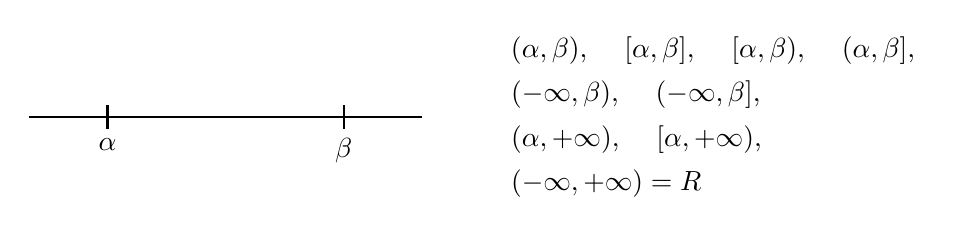
\begin{tikzpicture}
    % Recta (intervalo)
    \draw[thick] (0,0) -- (5,0);
    % Marca inicial alpha
    \draw[thick] (1,-0.15) -- (1,0.15);
    \node[below] at (1,-0.15) {$\alpha$};
    % Marca final beta
    \draw[thick] (4,-0.15) -- (4,0.15);
    \node[below] at (4,-0.15) {$\beta$};
    % Lista de intervalos a la derecha
    \node[right, align=left] at (6,0) {%
        $(\alpha, \beta)$, \quad $[\alpha, \beta]$, \quad $[\alpha, \beta)$, \quad $(\alpha, \beta]$,\\[4pt]
        $(-\infty, \beta)$, \quad $(-\infty, \beta]$,\\[4pt]
        $(\alpha, +\infty)$, \quad $[\alpha, +\infty)$,\\[4pt]
        $(-\infty, +\infty) = \mathbb{R}$%
    };
\end{tikzpicture}
\end{center}

Dada una función $f : J \times \Omega \to \mathbb{R}^n$, las nociones de Lipschitzianidad global y local se generalizan exigiendo que la acotación de las variaciones espaciales se cumpla de manera uniforme respecto a la variable temporal $t$.

\begin{definición}[Función global y localmente Lipschitziana en el caso no autónomo]
    Sea $J \subset \mathbb{R}$ un intervalo arbitrario, $\Omega \subset \mathbb{R}^n$ un conjunto abierto, y sea $f : J \times \Omega \to \mathbb{R}^n$ una función dada.
    \begin{enumerate}
        \item Se dice que $f$ es \textbf{globalmente Lipschitziana respecto de $u$ en $\Omega$}, uniformemente en $t \in J$, si existe una constante de Lipschitz $L > 0$ tal que:
        \[
            \| f(t, u) - f(t, v) \| \leq L \| u - v \|, \quad \forall t \in J, \; \forall u, v \in \Omega
        \]
        \item Se dice que $f$ es \textbf{localmente Lipschitziana respecto de $u$ en $\Omega$}, uniformemente en $t \in J$, si para cada $u_0 \in \Omega$ existen un radio $R > 0$ y una constante $L > 0$ (que puede depender de $u_0$) tales que la bola $B_R(u_0) \subset \Omega$ y se cumple:
        \[
            \| f(t, u) - f(t, v) \| \leq L \| u - v \|, \quad \forall t \in J, \; \forall u, v \in B_R(u_0)
        \]
    \end{enumerate}
\end{definición}

Al igual que en el caso autónomo, verificar esta condición mediante la definición directa puede ser tedioso. El siguiente teorema establece un criterio analítico equivalente basado en la acotación de las derivadas parciales respecto a las variables espaciales.

\begin{teorema}[Criterio de Lipschitzianidad para funciones no autónomas]
    Sean $J \subset \mathbb{R}$ un intervalo arbitrario, $\Omega \subset \mathbb{R}^n$ un conjunto abierto y \textbf{convexo}, y $f \in C (J \times \Omega, \mathbb{R}^n)$ una función que posee derivadas parciales $f_1, \ldots, f_n$ continuas. Es decir:
    \[
        \frac{\partial f_i}{\partial u_j} \in C(J \times \Omega, \mathbb{R}), \quad 1 \leq i,j \leq n
    \]
    Entonces, la función $f$ es globalmente Lipschitziana respecto a $u \in \Omega$ uniformemente en $t \in J$ si y solo si sus derivadas parciales están acotadas en todo el dominio. Esto se expresa como:
    \[
        f \text{ es globalmente Lipschitz. en } u 
        \iff
        M = \sup_{(t,u) \in J \times \Omega} \left| \frac{\partial f_i}{\partial u_j}(t,u) \right| < +\infty, \quad \forall i,j \in \{1, \ldots, n\}
    \]
\end{teorema}

\begin{proof}
    Demostraremos ambas implicaciones:
    \begin{itemize}
        \item[$\Leftarrow$] Supongamos que las derivadas parciales están acotadas por una constante $M < +\infty$. Fijados un instante $t \in J$ y dos puntos $u, v \in \Omega$, definimos la curva auxiliar $\varphi : [0,1] \to \mathbb{R}^n$ como:
        \[
            \varphi(s) = f(t, su + (1-s)v), \quad s \in [0,1]
        \]
        Como $\Omega$ es un conjunto convexo, el segmento de recta que une $u$ y $v$ está contenido íntegramente en $\Omega$, garantizando que la función $\varphi$ esté bien definida para todo $s \in [0,1]$. Aplicando el Teorema Fundamental del Cálculo y la regla de la cadena, obtenemos:
        \[
            \| f(t,u) - f(t,v) \| = \| \varphi(1) - \varphi(0) \| = \left\| \int_0^1 \varphi'(s) ds \right\| \leq \int_0^1 \| \varphi'(s) \| ds
        \]
        La derivada de la curva respecto al parámetro $s$ es $\varphi'(s) = D_u f(t, su + (1-s)v) \cdot (u - v)$, donde $D_u f$ representa la matriz jacobiana respecto a las variables espaciales $u$. Empleando la definición de la norma de operador matricial $\| \cdot \|_{\mathcal{L}(\mathbb{R}^n)}$:
        \[
            \| \varphi'(s) \| = \| D_u f(t, su + (1-s)v) \cdot (u - v) \| \leq \| D_u f(t, su + (1-s)v) \|_{\mathcal{L}(\mathbb{R}^n)} \| u - v \|
        \]
        En un espacio de dimensión finita todas las normas son equivalentes, por lo que existe una constante $c > 0$ tal que la norma de operador queda acotada por la suma de los valores absolutos de los elementos de la matriz. Dado que cada derivada parcial está acotada por $M$:
        \[
            \| D_u f(t, \dots) \|_{\mathcal{L}(\mathbb{R}^n)} \leq c \sum_{i,j=1}^n \left| \frac{\partial f_i}{\partial u_j} \right| \leq c \sum_{i,j=1}^n M = c n^2 M = L
        \]
        Sustituyendo esta constante $L$ en la integral obtenemos:
        \[
            \| f(t,u) - f(t,v) \| \leq \int_0^1 L \| u - v \| ds = L \| u - v \|
        \]
        Esto prueba que $f$ es globalmente Lipschitziana respecto a $u$, uniformemente en $t \in J$.

        \item[$\Rightarrow$] Supongamos ahora que existe una constante $L \geq 0$ tal que:
        \[
            \|f(t,u) - f(t,v)\| \leq L \|u - v\|, \quad \forall u, v \in \Omega, \quad \forall t \in J
        \]
        Fijados $t \in J$ y $u \in \Omega$, seleccionamos un vector dirección arbitrario $y \in \mathbb{R}^n$ con norma unidad ($\|y\|=1$). La derivada direccional de $f$, equivalente al producto de la matriz jacobiana por dicho vector, viene dada por:
        \[
            D_u f(t,u) y = \lim_{h \to 0} \frac{f(t, u+hy) - f(t,u)}{h}
        \]
        Utilizando la hipótesis de Lipschitzianidad, acotamos la norma del cociente incremental:
        \[
            \left\| \frac{f(t, u+hy) - f(t,u)}{h} \right\| = \frac{\|f(t, u+hy) - f(t,u)\|}{|h|} \leq \frac{L \|hy\|}{|h|} = \frac{L |h| \|y\|}{|h|} = L
        \]
        Tomando el límite cuando $h \to 0$, se deduce que $\|D_u f(t,u) y\| \leq L$ para todo vector unitario $y$. En consecuencia, la norma de operador de la matriz jacobiana satisface:
        \[
            \|D_u f(t,u)\|_{\mathcal{L}(\mathbb{R}^n)} = \max_{\|y\|=1} \|D_u f(t,u) y\| \leq L
        \]
        Por la equivalencia de normas, el valor absoluto de cada entrada de la matriz está acotado proporcionalmente por su norma de operador. Es decir, existe una constante $C > 0$ tal que:
        \[
            \left| \frac{\partial f_i}{\partial u_j} (t,u) \right| \leq C \|D_u f(t,u)\|_{\mathcal{L}(\mathbb{R}^n)} \leq C L
        \]
        Como esta cota superior es independiente tanto de $t$ como de $u$, concluimos que el supremo $M$ de las derivadas parciales en $J \times \Omega$ es finito.
    \end{itemize}
\end{proof}

\begin{corolario}
    Sean $J = [\alpha, \beta]$ un intervalo cerrado y acotado ($\alpha < \beta$), $\Omega \subset \mathbb{R}^n$ un conjunto abierto, y $f \in C(J \times \Omega, \mathbb{R}^n)$ una función tal que todas sus derivadas parciales $\frac{\partial f_i}{\partial u_j}$ son continuas en $J \times \Omega$. Entonces, para cada conjunto abierto, convexo y acotado $D \subset \Omega$ cuya clausura cumpla $\overline{D} \subset \Omega$, la función $f(t,u)$ es globalmente Lipschitziana respecto a $u \in D$, uniformemente en $t \in J$. En particular, $f$ es localmente Lipschitziana respecto a $u$ en $\Omega$, uniformemente en $t \in J$. 
\end{corolario}

\begin{proof}
    Sea $D \subset \Omega$ un subconjunto abierto, convexo y acotado con $\overline{D} \subset \Omega$. Por el teorema de Heine-Borel, al ser $\overline{D}$ un conjunto cerrado y acotado en $\mathbb{R}^n$, es compacto. Puesto que el intervalo $J$ también es compacto, el producto cartesiano $J \times \overline{D}$ resulta ser un conjunto compacto en $\mathbb{R} \times \mathbb{R}^n$.
    
    Como las derivadas parciales $\frac{\partial f_i}{\partial u_j}$ son funciones continuas en el conjunto compacto $J \times \overline{D}$, el teorema de Weierstrass garantiza que alcanzan valores extremos absolutos. En particular, están acotadas superiormente, por lo que existe una constante $M > 0$ tal que:
    \[
        \sup_{(t,u) \in J \times D} \left| \frac{\partial f_i}{\partial u_j}(t,u) \right| \leq M, \quad \forall i,j \in \{1, \ldots, n\}
    \]
    En virtud del teorema anterior, esta acotación uniforme de las derivadas implica que $f$ es globalmente Lipschitziana respecto a $u \in D$, uniformemente en $t \in J$. Dado que todo punto $u_0 \in \Omega$ admite un entorno que satisface las propiedades del conjunto $D$, se concluye que $f$ es localmente Lipschitziana en todo el dominio $\Omega$.
\end{proof}

\ejemplo{
    \begin{enumerate}
        \item Sea la función:
        \[
            f(t,u) = a(t) \sin(u), \quad u \in \mathbb{R}, \quad t \in [\alpha, \beta], \quad a \in C([\alpha, \beta], \mathbb{R})   
        \]
        Su derivada parcial respecto a $u$ es:
        \[
            \frac{\partial f}{\partial u}(t,u) = a(t) \cos(u)
        \]
        Esta derivada es continua. Acotando su valor absoluto para todo $(t,u) \in [\alpha, \beta] \times \mathbb{R}$:
        \[
            \left| \frac{\partial f}{\partial u} (t,u) \right| = |a(t)| |\cos(u)| \leq |a(t)| \leq \max_{t \in [\alpha, \beta]} |a(t)| = M < +\infty
        \]
        El máximo existe porque $a(t)$ es continua en el compacto $[\alpha, \beta]$. Al estar la derivada global y uniformemente acotada, la función $f$ es globalmente Lipschitziana respecto a $u \in \mathbb{R}$, uniformemente en $t \in [\alpha, \beta]$.

        \item Sea la función con una singularidad temporal en el origen:
        \[
            f(t,u) = \frac{1}{t} \sin(u), \quad u \in \mathbb{R}, \quad t \in J = (0, \infty)
        \]
        La derivada parcial respecto a $u$ es:
        \[
            \frac{\partial f}{\partial u}(t,u) = \frac{1}{t} \cos(u)
        \]
        Calculando el supremo respecto a $u$ para un $t$ fijo:
        \[
            \sup_{u \in \mathbb{R}} \left| \frac{\partial f}{\partial u} (t,u) \right| = \frac{1}{t}
        \]
        Al tomar el límite cuando $t \to 0^+$, este supremo diverge a $+\infty$. Dado que la derivada parcial no está acotada uniformemente en el intervalo $J$, la función $f$ no es globalmente Lipschitziana respecto a $u$ uniformemente en $J$. 

        \item Sea la función con crecimiento polinomial:
        \[
            f(t,u) = a(t) |u|^p, \quad u \in \mathbb{R}, \quad t \in [\alpha, \beta], \quad a \in C([\alpha, \beta], \mathbb{R})
        \]
        donde $p > 1$. Su derivada parcial respecto a $u$ para $u \neq 0$ es:
        \[
            \frac{\partial f}{\partial u}(t,u) = a(t) p |u|^{p-1} \operatorname{sgn}(u)
        \]
        (Puesto que $p > 1$, la derivada en $u=0$ existe y es nula, por lo que la función derivada resulta continua en todo $\mathbb{R}$). Sin embargo, al fijar un instante $t$ donde $a(t) \neq 0$, el término $|u|^{p-1}$ diverge a $+\infty$ cuando $|u| \to \infty$. Esto implica que la derivada no está acotada globalmente en $\mathbb{R}$. Por consiguiente, $f$ no es globalmente Lipschitziana en el espacio completo. No obstante, por aplicación directa del corolario anterior, la función sí es localmente Lipschitziana respecto a $u$, uniformemente en $t \in [\alpha, \beta]$.
        \item Sea la función matricial:
        \[
            f(t,u) = A(t) u + B(t), \quad
            \begin{cases}
                A(t) = (a_{ij}(t))_{1 \leq i,j \leq n} \\
                B(t) = (b_i(t))_{1 \leq i \leq n} \\
                a_{ij}, b_i \in C([\alpha, \beta], \mathbb{R})
            \end{cases}
        \]
        Ahora nótese que podemos calcular cada $f_i$ como:
        \[
            f_i(t,u) = \sum_{k=1}^n a_{ik}(t) u_k + b_i(t), \quad 1 \leq i \leq n
        \]
        Y además $f \in C([\alpha, \beta] \times \mathbb{R}^n, \mathbb{R}^n)$ si fijamos $\Omega = \mathbb{R}^n$. Las derivadas parciales respecto a cada $u_j$ son, $\forall t \in [\alpha, \beta]$, $\forall i,j \in \{1, \ldots, n\}$:
        \[
            \left| \frac{\partial f_i}{\partial u_j}(t,u) \right| = 
            |a_{ij}(t)| \leq 
            \max_{t \in [\alpha, \beta]} |a_{ij}(t)| = 
            \| a_{ij} \|_\infty < +\infty
        \]
        Y por lo tanto, todas las derivadas parciales están uniformemente acotadas en $[\alpha, \beta] \times \mathbb{R}^n$. En consecuencia, la función $f$ es globalmente Lipschitziana respecto a $u \in \mathbb{R}^n$, uniformemente en $t \in [\alpha, \beta]$.
        \item Sea la función matricial:
        \[
            f(t,u) = A(t) 
            \begin{pmatrix}
                \sin(u_1) \\
                \vdots \\
                \sin(u_n)
            \end{pmatrix}
            + B(t) 
        \]
        Donde $A(t)$ y $B(t)$ son continuas en $[\alpha, \beta]$. Cada $f_i$ se puede expresar como:
        \[
            f_i(t,u) = 
            \sum_{k=1}^n a_{ik}(t) \sin(u_k) + b_i(t), \quad 1 \leq i \leq n
        \]
        Que son además continuas en $[\alpha, \beta] \times \mathbb{R}^n$. Las derivadas parciales respecto a cada $u_j$ son:
        \[
            \left| \frac{\partial f_i}{\partial u_j}(t,u) \right| = 
            |a_{ij}(t)| |\cos(u_j)| \leq 
            |a_{ij}(t)| \leq 
            \max_{t \in [\alpha, \beta]} |a_{ij}(t)| = 
            \| a_{ij} \|_\infty < +\infty
        \]
        Por lo tanto, todas las derivadas parciales están uniformemente acotadas en $[\alpha, \beta] \times \mathbb{R}^n$, y la función $f$ es globalmente Lipschitziana respecto a $u \in \mathbb{R}^n$, uniformemente en $t \in [\alpha, \beta]$.\\
        Si las matrices $A(t)$ y $B(t)$ son continuas en todo $\mathbb{R}$, la función $f$ localmente Lipschitziana respecto a $u$ en $\mathbb{R}^n$, uniformemente en $t \in \mathbb{R}$, ya que en cualquier intervalo compacto de tiempo $[\alpha, \beta]$ se cumple la condición de Lipschitzianidad global, pero puede que no se cumpla la acotación global en todo $\mathbb{R}$.
        \item Sea la función:
        \[
            f(t,u) = A(t)
            \begin{pmatrix}
                |u_1|^{p_1} \\
                \vdots \\
                |u_n|^{p_n}
            \end{pmatrix}
            + B(t), \quad p_i > 1, \quad 1 \leq i \leq n
        \]
        Con además $A(t)$ y $B(t)$ continuas en $[\alpha, \beta]$. Cada $f_i$ se puede expresar como:
        \[
            f_i(t,u) = 
            \sum_{k=1}^n a_{ik}(t) |u_k|^{p_k} + b_i(t) \in C([\alpha, \beta] \times \mathbb{R}^n, \mathbb{R})
            , \quad 1 \leq i \leq n
        \]
        Que son además continuas en $[\alpha, \beta] \times \mathbb{R}^n$. Las derivadas parciales respecto a cada $u_j$ son:
        \[
            \left| \frac{\partial f_i}{\partial u_j}(t,u) \right| = 
            |a_{ij}(t)| p_j |u_j|^{p_j - 1}
        \]
        Debido al corolario, es trivial ver que esta función es localmente Lipschitziana respecto a $u$ en $\mathbb{R}^n$, uniformemente en $t \in [\alpha, \beta]$. Sin embargo, si $A(t) \neq 0$, entonces existen $i_0, j_0, t_0$ tales que $a_{i_0 j_0}(t_0) \neq 0$. En este caso, la derivada parcial $\frac{\partial f_{i_0}}{\partial u_{j_0}}(t_0,u)$ diverge a $+\infty$:
        \[
            \left| \frac{\partial f_{i_0}}{\partial u_{j_0}}(t_0,u) \right| = |a_{i_0 j_0}(t_0)| p_{j_0} |u_{j_0}|^{p_{j_0} - 1} \xrightarrow{|u_{j_0}| \to \infty}_{p_{j_0} - 1 > 0} +\infty
        \]
        Demostrando que la función no es globalmente Lipschitziana respecto a $u$ en $\mathbb{R}^n$, uniformemente en $t \in [\alpha, \beta]$, al tener una derivada parcial no acotada en el dominio completo.
    \end{enumerate}
}

\subsubsection{Teorema fundamental global de Cauchy-Lipschitz}

\begin{teorema}[Teorema fundamental global de Cauchy-Lipschitz]
    Sean $N \geq 1$, $\alpha < \beta$, y $f \in C([\alpha, \beta] \times \mathbb{R}^N, \mathbb{R}^N)$ una función globalmente Lipschitziana respecto a $u \in \mathbb{R}^N$, uniformemente en $t \in [\alpha, \beta]$. Es decir, existe una constante $L \geq 0$ tal que:
    \[
        \| f(t,u) - f(t,v) \| \leq L \| u - v \|, \quad \forall t \in [\alpha, \beta], \quad \forall u, v \in \mathbb{R}^N
    \]
    Entonces, para cada $t_0 \in [\alpha, \beta]$ y cada $u_0 \in \mathbb{R}^N$, el problema de valor inicial (PVI):
    \[
        (P) \quad
        \begin{cases}
            u'(t) = f(t, u(t)), \quad t \in [\alpha, \beta] \\
            u(t_0) = u_0
        \end{cases}
    \]
    el cual denotaremos habitualmente de forma abreviada como $u' = f(t,u)$ con $u(t_0) = u_0$, tiene una única solución globalmente definida en todo el intervalo $[\alpha, \beta]$, la cual se denota por:
    \[
        u(t) = u(t; t_0, u_0), \quad t \in [\alpha, \beta]
    \]
\end{teorema}

\begin{proof}
    El problema de valor inicial $(P)$ consiste en encontrar una función $u \in C^1([\alpha, \beta]; \mathbb{R}^N)$ que satisfaga la ecuación diferencial y la condición inicial. 
    
    Como se ha visto en resultados previos de ecuaciones diferenciales, podemos integrar la ecuación $u'(s) = f(s, u(s))$ entre el instante inicial $t_0$ y un instante arbitrario $t$:
    \[
        \int_{t_0}^t u'(s) ds = \int_{t_0}^t f(s, u(s)) ds \implies u(t) - u(t_0) = \int_{t_0}^t f(s, u(s)) ds
    \]
    Por lo tanto, una función $u$ es solución de $(P)$ si y solo si $u \in C([\alpha, \beta]; \mathbb{R}^N)$ satisface la ecuación integral de Volterra equivalente:
    \[
        u(t) = u_0 + \int_{t_0}^t f(s, u(s)) ds, \quad \forall t \in [\alpha, \beta]
    \]
    A partir de esta formulación, definimos el operador integral de Picard $K : C([\alpha, \beta]; \mathbb{R}^N) \to C([\alpha, \beta]; \mathbb{R}^N)$ dado por:
    \[
        (Ku)(t) = u_0 + \int_{t_0}^t f(s, u(s)) ds
    \]
    Las soluciones del problema $(P)$ se corresponden exactamente con los puntos fijos del operador $K$. Para demostrar que existe un único punto fijo, utilizaremos el Teorema del Punto Fijo de Banach. 
    
    El espacio vectorial $X = C([\alpha, \beta]; \mathbb{R}^N)$ equipado con la norma del supremo es un espacio de Banach. Para facilitar las estimaciones y garantizar que $K$ sea una contracción, introducimos una norma equivalente conocida como la norma de Bielecki. Tomando un parámetro $\gamma > L$, definimos:
    \[
        \| u \|_B = \max_{t \in [\alpha, \beta]} e^{-\gamma |t - t_0|} \| u(t) \|
    \]
    Al ser equivalente a la norma del supremo, el espacio $(X, \| \cdot \|_B)$ sigue siendo un espacio de Banach. Evaluemos la distancia entre las imágenes de dos funciones $u, v \in X$ bajo el operador $K$. Asumiendo $t \geq t_0$, tenemos:
    \[
        \| (Ku)(t) - (Kv)(t) \| = \left\| \int_{t_0}^t \left( f(s, u(s)) - f(s, v(s)) \right) ds \right\| \leq \int_{\min(t_0, t)}^{\max(t_0, t)} \| f(s, u(s)) - f(s, v(s)) \| ds
    \]
    Aplicando la condición de Lipschitz global:
    \[
        \| (Ku)(t) - (Kv)(t) \| \leq L \int_{\min(t_0, t)}^{\max(t_0, t)} \| u(s) - v(s) \| ds
    \]
    Multiplicamos y dividimos el integrando por el factor exponencial $e^{\gamma(s - t_0)}$ para hacer aparecer la estructura de la norma de Bielecki:
    \[
        \| (Ku)(t) - (Kv)(t) \| \leq L \int_{\min(t_0, t)}^{\max(t_0, t)} e^{\gamma(s - t_0)} \left( e^{-\gamma(s - t_0)} \| u(s) - v(s) \| \right) ds
    \]
    Acotando el término entre paréntesis por la norma $\| u - v \|_B$:
    \[
        \| (Ku)(t) - (Kv)(t) \| \leq L \| u - v \|_B \int_{\min(t_0, t)}^{\max(t_0, t)} e^{\gamma(s - t_0)} ds = L \| u - v \|_B \left[ \frac{e^{\gamma(s - t_0)}}{\gamma} \right]_{t_0}^t \leq \frac{L}{\gamma} e^{\gamma(t - t_0)} \| u - v \|_B
    \]
    Multiplicando ambos lados por $e^{-\gamma(t - t_0)}$ se obtiene:
    \[
        e^{-\gamma|t - t_0|} \| (Ku)(t) - (Kv)(t) \| \leq \frac{L}{\gamma} \| u - v \|_B
    \]
    Un razonamiento simétrico aplicando propiedades de la integral para el caso $t \leq t_0$ conduce a la misma cota. Tomando el máximo sobre todo $t \in [\alpha, \beta]$, concluimos que:
    \[
        \| Ku - Kv \|_B \leq \frac{L}{\gamma} \| u - v \|_B
    \]
    Como hemos elegido $\gamma > L$, se cumple que $\frac{L}{\gamma} < 1$. Por lo tanto, el operador $K$ es una contracción estricta en el espacio de Banach $(X, \| \cdot \|_B)$. 
    
    Por el Teorema del Punto Fijo de Banach, el operador $K$ posee un único punto fijo $u \in X$. Esta función es la única solución global del problema de valor inicial en el intervalo $[\alpha, \beta]$.
\end{proof}

\begin{corolario}
    Como consecuencia directa de la aplicación del Teorema del Punto Fijo en la demostración anterior, para cada función continua $h_0 \in C([\alpha, \beta]; \mathbb{R}^N)$, la sucesión de funciones definida recursivamente mediante el operador integral:
    \[
        h_n(t) = K (h_{n-1})(t) = u_0 + \int_{t_0}^t f(s, h_{n-1}(s)) ds, \quad n \geq 1
    \]
    converge uniformemente en $[\alpha, \beta]$ hacia la única solución $u(t)$ del problema de valor inicial $(P)$.
\end{corolario}

A continuación, presentamos dos ejemplos de sistemas de ecuaciones diferenciales que satisfacen las hipótesis del teorema y, por consiguiente, poseen una única solución global.

\ejemplo{
    \begin{enumerate}
        \item \textbf{Sistema lineal no autónomo:}
        Consideramos el problema de valor inicial dado por:
        \[
            u'(t) = A(t) u(t) + B(t), \quad u(t_0) = u_0 \in \mathbb{R}^N, \quad t_0 \in [\alpha, \beta]
        \]  
        donde $A(t) = (a_{ij}(t))_{1 \leq i,j \leq N}$ y $B(t) = (b_i(t))_{1 \leq i \leq N}$, con coeficientes $a_{ij}, b_i \in C([\alpha, \beta], \mathbb{R})$. 
        Dado que las funciones $a_{ij}(t)$ son continuas en un intervalo compacto, alcanzan un valor máximo y están acotadas. Esto garantiza que la función $f(t,u) = A(t)u + B(t)$ sea globalmente Lipschitziana respecto a $u$, uniformemente en $t \in [\alpha, \beta]$. Por tanto, el problema tiene una única solución global.

        \item \textbf{Sistema no lineal con derivadas espaciales acotadas:}
        Sea el sistema definido por sus componentes:
        \[
            u_i'(t) = \sum_{j=1}^N a_{ij}(t) \sin(u_j(t)) + b_i(t), \quad 1 \leq i \leq N
        \]  
        con datos iniciales $u(t_0) = u_0$ y coeficientes $a_{ij}, b_i \in C([\alpha, \beta], \mathbb{R})$. 
        Las derivadas parciales de la función $f$ respecto a las variables espaciales $u_k$ son $a_{ik}(t) \cos(u_k)$. Como los coeficientes $a_{ik}(t)$ son continuos en el compacto $[\alpha, \beta]$ y el coseno está acotado por 1, todas las derivadas parciales están uniformemente acotadas. Aplicando el criterio de Lipschitzianidad visto anteriormente, $f$ es globalmente Lipschitziana respecto a $u$, asegurando la existencia de una única solución global en $[\alpha, \beta]$.
    \end{enumerate}
}

\begin{corolario}
    Sea $J \subset \mathbb{R}$ un intervalo abierto arbitrario, y $f \in C(J \times \mathbb{R}^N, \mathbb{R}^N)$ una función globalmente Lipschitziana respecto a $u \in \mathbb{R}^N$, uniformemente en $t \in J$. Entonces, para cada $t_0 \in J$ y cada $u_0 \in \mathbb{R}^N$, el problema de valor inicial:
    \[
        (P) \quad
        \begin{cases}
            u'(t) = f(t, u(t)), \quad t \in J \\
            u(t_0) = u_0
        \end{cases}
    \]
    tiene una única solución globalmente definida en todo el intervalo $J$, la cual se denota por:
    \[
        u(t) = u(t; t_0, u_0), \quad t \in J
    \]
\end{corolario}

\begin{proof}
    Dado que $J$ es un intervalo abierto, existe una sucesión de intervalos cerrados y acotados $\{J_n\}_{n \geq 1}$ que forman una cadena creciente y cuya unión recubre todo $J$. Es decir:
    \[
        J_1 \subset J_2 \subset \ldots \subset J_n \subset \ldots, \quad \bigcup_{n \geq 1} J_n = J
    \]
    Por ejemplo, si $J = (\alpha, \beta)$, basta tomar $J_n = [\alpha + \frac{1}{n}, \beta - \frac{1}{n}]$ para valores de $n$ suficientemente grandes. Construcciones análogas aplican si $J = \mathbb{R}$ tomando $J_n = [-n, n]$, o en intervalos no acotados como $J = (\alpha, \infty)$ tomando $J_n = [\alpha + \frac{1}{n}, n]$.

    Fijado el tiempo inicial $t_0 \in J$, existe un índice $n_0 \geq 1$ tal que $t_0 \in J_n$ para todo $n \geq n_0$. Consideremos la restricción del problema de valor inicial a un intervalo compacto genérico $J_n$ (con $n \geq n_0$):
    \[
        \begin{cases}
            u'(t) = f(t, u(t)), \quad t \in J_n \\
            u(t_0) = u_0
        \end{cases}
    \]
    Al cumplir $f$ la condición de Lipschitz uniformemente en todo $J$, también la cumple en $J_n$. Por el Teorema fundamental global de Cauchy-Lipschitz, para cada $n \geq n_0$ existe una única solución $u_n(t)$ definida en el intervalo $J_n$. 
    
    Si consideramos un índice $m > n$, la función $u_m(t)$ es la solución única en $J_m$. Su restricción al subintervalo $J_n$ sigue satisfaciendo la ecuación diferencial y el dato inicial, por lo que, debido a la unicidad en $J_n$, se concluye que $u_m(t) = u_n(t)$ para todo $t \in J_n$. Este hecho permite definir una función $u : J \to \mathbb{R}^N$ de manera consistente en todo el dominio $J$:
    \[
        u(t) = u_n(t), \quad \text{donde } n \geq n_0 \text{ es cualquier índice tal que } t \in J_n
    \]
    La función $u(t)$ está bien definida y es solución del problema $(P)$ en $J$. Para verificar su unicidad, supongamos que existe otra solución $v : J \to \mathbb{R}^N$. Si ambas difirieran en algún punto $t_1 \in J$, existiría un índice $k \geq n_0$ tal que $t_1 \in J_k$. Sin embargo, al restringir ambas funciones a $J_k$, tendríamos dos soluciones distintas para el mismo problema de valor inicial en un intervalo compacto, lo cual contradice el teorema fundamental. Por tanto, $u(t) = v(t)$ para todo $t \in J$.
\end{proof}

\textbf{Observación sobre el relajamiento de hipótesis.} Del proceso de construcción mediante compactos exhaustivos (sucesión $J_n$) empleado en la demostración anterior, se extrae un hecho de gran utilidad práctica. Como el Teorema fundamental global solo se aplica localmente sobre cada compacto $J_n$, no es necesario que la constante de Lipschitz de la función $f$ sea la misma en todo $J$. 

Basta exigir que $f$ sea globalmente Lipschitziana respecto a $u$ en $\mathbb{R}^N$ \textit{uniformemente sobre cada subintervalo compacto} $[\alpha, \beta] \subset J$. Esta condición relajada es suficiente para asegurar la existencia y unicidad en cada $J_n$, permitiendo extender la solución a todo $J$ y ampliando la clase de problemas que admiten solución global.

\ejemplo{
    Consideremos el siguiente problema de valor inicial autónomo:
    \[
        \begin{cases}
            u'(t) = u(t)^2 \\
            u(0) = u_0 > 0
        \end{cases}   
    \]
    La función $f(t,u) = u^2$ es localmente Lipschitziana respecto a $u$ en $\mathbb{R}$, uniformemente en $t \in \mathbb{R}$. Sin embargo, como se vio en ejemplos anteriores, su derivada parcial $\frac{\partial f}{\partial u} = 2u$ no está acotada en todo $\mathbb{R}$, por lo que la función no satisface la condición de Lipschitz global.

    Para resolver la ecuación diferencial explícitamente, separamos las variables. Como $u_0 > 0$, la solución será no nula en un entorno de $t=0$, lo que nos permite dividir la ecuación por $u^2$:
    \[
        u^{-2} u' = 1 \implies -\frac{d}{dt} \left( u^{-1} \right) = 1
    \]
    Integrando con respecto a la variable temporal $t$, obtenemos:
    \[
        -\frac{1}{u(t)} = t - c \implies \frac{1}{u(t)} = -t + c
    \]
    Imponiendo la condición inicial $u(0) = u_0$, determinamos la constante de integración $c$:
    \[
        \frac{1}{u(0)} = c \implies c = \frac{1}{u_0}
    \]
    Sustituyendo el valor de la constante y operando para despejar $u(t)$:
    \[
        \frac{1}{u(t)} = -t + \frac{1}{u_0} = \frac{1 - t u_0}{u_0} \implies u(t) = \frac{u_0}{1 - t u_0}
    \]
    Analizando el dominio de esta solución, observamos que el denominador se anula en el instante $t = 1/u_0$. Dado que $u_0 > 0$, este valor corresponde a un tiempo futuro positivo. Por consiguiente, si consideramos el avance temporal desde $t=0$, la solución está definida únicamente en el intervalo $[0, 1/u_0)$. 
    
    Cuando el tiempo se aproxima al valor $1/u_0$, la solución diverge:
    \[
        \lim_{t \to (1/u_0)^-} u(t) = +\infty
    \]
    Este comportamiento se conoce como explosión en tiempo finito (\textit{blow-up}). El ejemplo ilustra que, cuando una función carece de la condición de Lipschitz global y solo posee Lipschitzianidad local, no se puede garantizar la existencia global de la solución en todo el intervalo temporal de definición, justificando así la necesidad de las hipótesis del teorema fundamental global.
}

\subsubsection{ Teorema local de Cauchy-Lipschitz}

\begin{teorema}[Teorema local de Cauchy-Lipschitz]
    Sean $t_0 \in \mathbb{R}$, $T > 0$, y consideremos el intervalo temporal $J = [t_0, t_0 + T]$. Sea $\Omega \subset \mathbb{R}^N$ un conjunto abierto y $f \in C(J \times \Omega, \mathbb{R}^N)$ una función localmente Lipschitziana respecto a $u \in \Omega$, uniformemente en $t \in J$. Entonces, para cada $u_0 \in \Omega$, el problema de valor inicial:
    \[
        (P) \quad
        \begin{cases}
            u'(t) = f(t, u(t)), \quad t \in J \\
            u(t_0) = u_0
        \end{cases}
    \]
    admite una única solución local. De manera más precisa:
    \begin{enumerate}
        \item Existe $\delta \in (0, T]$ tal que el problema $(P)$ tiene una única solución $u \in C^1([t_0, t_0 + \delta], \mathbb{R}^N)$.
        \item Si consideramos una bola cerrada $\overline{B}_R(u_0) = \{u \in \mathbb{R}^N : \| u - u_0 \|_2 \leq R\} \subset \Omega$ tal que $f$ es globalmente Lipschitziana respecto a $u$ en dicha bola (uniformemente en $t \in J$), y definimos la cota del supremo:
        \[
            M = \| f \|_\infty = \max_{(t,u) \in J \times \overline{B}_R(u_0)} \| f(t,u) \|_2
        \]
        junto con el intervalo temporal de validez garantizada:
        \[
            \delta_0 = \min \left\{ T, \frac{R}{M} \right\}
        \]
        entonces el problema $(P)$ tiene una única solución $u \in C^1([t_0, t_0 + \delta_0], \mathbb{R}^N)$.
    \end{enumerate}
    Además, podemos definir un problema alternativo:
    \[
        (P_F) \quad
        \begin{cases}
            u'(t) = F(t, u(t)), \quad t \in J \\
            u(t_0) = u_0
        \end{cases}
    \]
    Dónde:
    \[
        F(t,u) = \begin{cases}
            f(t,u), & \text{si } u \in \overline{B}_R(u_0) \\
            f(t, \tilde{u}), & \text{si } u \notin \overline{B}_R(u_0)
        \end{cases}
        \, \quad
        \tilde{u} = u_0 + R \frac{u - u_0}{\| u - u_0 \|_2}
    \]
    % Dibujo con u_0, u y tilde u
    \begin{center}
        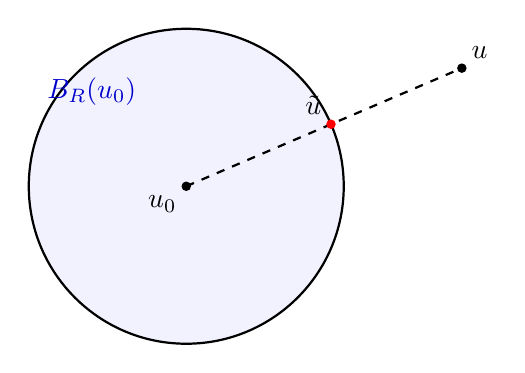
\begin{tikzpicture}
            % Dibujamos la bola
            \draw[thick, fill=blue!5] (0,0) circle (2cm);
            
            % Coordenadas
            \coordinate (u0) at (0,0);
            \coordinate (u) at (3.5, 1.5);
            % Intersección exacta: (2*3.5/3.80788, 2*1.5/3.80788)
            \coordinate (utilde) at (1.838, 0.788); 
            
            % Línea punteada desde el centro hasta u
            \draw[dashed, thick] (u0) -- (u);
            
            % Puntos y etiquetas
            \filldraw[black] (u0) circle (1.5pt) node[below left] {$u_0$};
            \filldraw[black] (u) circle (1.5pt) node[above right] {$u$};
            \filldraw[red] (utilde) circle (1.5pt) node[above left, text=black] {$\tilde{u}$};
            
            % Etiqueta de la bola
            \node[blue!80!black] at (-1.2, 1.2) {$B_R(u_0)$};
        \end{tikzpicture}
    \end{center}
    
\end{teorema}

\begin{proof}
    La demostración se estructura en tres etapas lógicas: primero, modificaremos el problema para garantizar una solución global (Etapa 1); luego, demostraremos que cualquier solución local original no escapa de cierta bola, probando así la unicidad (Etapa 2); y finalmente, comprobaremos que la solución global construida se restringe válidamente a nuestro intervalo de interés sin salir de dicha bola, asegurando la existencia (Etapa 3).

    \subsection*{Etapa 1}
    Acometeremos la prueba estableciendo primero un problema modificado con existencia global, para luego demostrar que su solución coincide localmente con la del problema original $(P)$.
    
    Definimos una función auxiliar $F : J \times \mathbb{R}^N \to \mathbb{R}^N$ que extienda a $f$ fuera de la bola $\overline{B}_R(u_0)$ de forma constante a lo largo de las direcciones radiales:
    \[
        F(t,u) = \begin{cases}
            f(t,u), & \text{si } \| u - u_0 \|_2 \leq R \\
            f(t, \tilde{u}), & \text{si } \| u - u_0 \|_2 > R
        \end{cases}
    \]
    donde $\tilde{u} = u_0 + R \frac{u - u_0}{\| u - u_0 \|_2}$ es la proyección radial del punto $u$ sobre la frontera de la bola (la esfera de radio $R$ centrada en $u_0$). Al ser $f$ continua y la proyección también continua, $F$ es una función continua en todo $J \times \mathbb{R}^N$. 
    
    Comprobemos que $F$ es globalmente Lipschitziana respecto a $u$ en todo $\mathbb{R}^N$, con la misma constante $L$ que $f$ posee en la bola cerrada. Se presentan tres casos para $u, v \in \mathbb{R}^N$:
    \begin{enumerate}
        \item Si $u, v \in \overline{B}_R (u_0)$, entonces $F$ coincide con $f$ y la desigualdad se verifica directamente:
        \[
            \| F(t,u) - F(t,v) \|_2 = \| f(t,u) - f(t,v) \|_2 \leq L \| u - v \|_2
        \]
        \item Si $\| u - u_0 \|_2 \leq R$ pero $\| v - u_0 \|_2 > R$, evaluamos $F$ usando la proyección $\tilde{v}$. Puesto que la proyección radial sobre un conjunto convexo es una contracción (es decir, $\| u - \tilde{v} \|_2 \leq \| u - v \|_2$), resulta:
        \[
            \| F(t,u) - F(t,v) \|_2 = \| f(t,u) - f(t, \tilde{v}) \|_2 \leq L \| u - \tilde{v} \|_2 \leq L \| u - v \|_2
        \]
        \item Si ambos puntos son exteriores a la bola ($\| u - u_0 \|_2 > R$ y $\| v - u_0 \|_2 > R$), evaluamos en las proyecciones $\tilde{u}$ y $\tilde{v}$. Por la misma propiedad de contracción de la proyección radial:
        \[
            \| F(t,u) - F(t,v) \|_2 = \| f(t, \tilde{u}) - f(t, \tilde{v}) \|_2 \leq L \| \tilde{u} - \tilde{v} \|_2 \leq L \| u - v \|_2
        \]
    \end{enumerate} 
    
    Queda probado que $F$ es globalmente Lipschitziana en todo $\mathbb{R}^N$, uniformemente en $J$. En virtud del Teorema fundamental global de Cauchy-Lipschitz, el problema de valor inicial modificado:
    \[
        (P_F) \quad \begin{cases}
            U'(t) = F(t, U(t)), \quad t \in J \\
            U(t_0) = u_0
        \end{cases}
    \]
    posee una única solución global $U \in C^1(J, \mathbb{R}^N)$.
    
    A continuación, evaluaremos hasta qué instante temporal $t$ esta solución $U(t)$ permanece dentro de la bola $\overline{B}_R(u_0)$. Mientras $U(t) \in \overline{B}_R(u_0)$, la función $F$ coincide idénticamente con $f$, por lo que $U(t)$ será también solución del problema original $(P)$.
    
    Tomemos un $t > t_0$ asumiendo que la solución se mantiene en la bola en el intervalo $[t_0, t]$. Aplicando la ecuación integral equivalente al PVI y tomando normas:
    \[
        \| U(t) - u_0 \|_2 = \left\| \int_{t_0}^t F(s, U(s)) ds \right\|_2 \leq \int_{t_0}^t \| F(s, U(s)) \|_2 ds
    \]
    Como $U(s) \in \overline{B}_R(u_0)$ para $s \in [t_0, t]$, sabemos que $F(s, U(s)) = f(s, U(s))$. Además, la norma de $f$ en la bola está acotada superiormente por $M = \| f \|_\infty$. Sustituyendo esta cota:
    \[
        \| U(t) - u_0 \|_2 \leq \int_{t_0}^t M ds = M (t - t_0)
    \]
    Para garantizar que la solución no escape de la bola, debemos asegurar que la distancia al centro no supere $R$, lo que requiere $M (t - t_0) \leq R$. Despejando, la condición se cumple siempre que:
    \[
        t - t_0 \leq \frac{R}{M}
    \]
    Considerando que el dominio temporal está restringido a longitud $T$, el intervalo máximo asegurado para la permanencia en la bola viene dado por $\delta_0 = \min \left\{ T, \frac{R}{M} \right\}$, nótese que si $M=\| f \|_\infty = 0$, entonces tomaríamos $\delta_0 = T$ y la solución permanecería en la bola durante todo el intervalo.
    
    Por consiguiente, para todo $t \in [t_0, t_0 + \delta_0]$, se cumple $\| U(t) - u_0 \|_2 \leq R$. En todo este subintervalo, el sistema modificado $(P_F)$ coincide con el sistema original $(P)$, y la solución $U(t)$ resuelve $(P)$. 
    
    Para concluir la unicidad, sea $u(t)$ cualquier otra solución de $(P)$ definida en $[t_0, t_0 + \delta_0]$. Por continuidad, existe un intervalo maximal donde $u(t) \in \overline{B}_R(u_0)$. Mediante el mismo razonamiento integral previo, el tiempo requerido para que la solución abandone la bola es estrictamente mayor que $\delta_0$. Así, $u(t)$ nunca abandona la bola en $[t_0, t_0 + \delta_0]$. Como consecuencia, $u(t)$ también es solución de $(P_F)$ en ese intervalo. Dada la unicidad global de las soluciones de $(P_F)$, deducimos que $u(t) \equiv U(t)$ en $[t_0, t_0 + \delta_0]$.

    \subsection*{Etapa 2}

    Siempre que $u(t)$ sea una solución de $(P)$ en un intervalo $[t_0, t_0 + \delta]$ con $\delta \leq \delta_0$, se cumple que $u(t) \in \overline{B}_R(u_0)$, $\forall t \in [t_0, t_0 + \delta]$.\\

    Por reducción al absurdo, supongamos que $\exists \widetilde{t} \in [t_0, t_0 + \delta]$ tal que $\| u(\widetilde{t}) - u_0 \|_2 > R$, pero esto implicaría:
    \[
        \exists t_1 \in [t_0, \widetilde{t}) \text{ tal que } 
        \begin{cases}
            \| u(t) - u_0 \|_2 < R \text{ si } t_0 \leq t < t_1 \\
            \| u(t_1) - u_0 \|_2 = R
        \end{cases}
    \]

    Por lo que podemos deducir que:
    \[
        R = \| u(t_1) - u_0 \|_1 =
        \left\| \int_{t_0}^{t_1} u'(s) ds \right\|_1 =
        \left\| \int_{t_0}^{t_1} f(s, u(s)) ds \right\|_1 \leq
        \int_{t_0}^{t_1} \| f(s, u(s)) \|_1 ds \leq
        \| f \|_\infty (t_1 - t_0) \implies
    \]
    \[
        \implies
        t_1 - t_0 \geq \frac{R}{\| f \|_\infty} \implies
        t_1 \geq t_0 + \frac{R}{\| f \|_\infty} \geq t_0 + \delta_0 \equiv
        \boxed{t_1 \geq t_0 + \delta_0 !!}
    \]
    Habiendo así reducido al absurdo, se concluye que $\| u(t) - u_0 \|_2 \leq R$ para todo $t \in [t_0, t_0 + \delta]$, y por lo tanto $u(t)$ es también solución de $(P_F)$ en ese intervalo. Por la unicidad de la solución de $(P_F)$, se deduce que $u(t) \equiv U(t)$ en $[t_0, t_0 + \delta]$.\\

    Un dibujo que nos puede ayudar a entender esta demostración es el siguiente:
    \begin{center}
        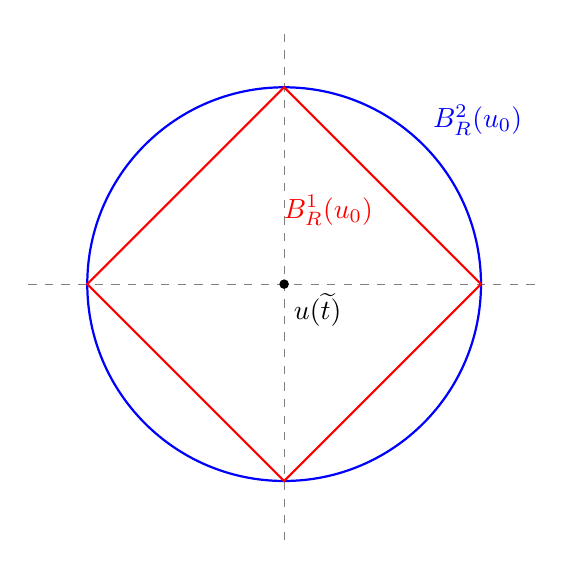
\begin{tikzpicture}[scale=2.5]
            % Rectas horizontal y vertical discontinuas
            \draw[dashed, gray] (-1.3, 0) -- (1.3, 0);
            \draw[dashed, gray] (0, -1.3) -- (0, 1.3);

            % Bola bajo la norma 2 (círculo)
            \draw[thick, blue] (0,0) circle (1);
            \node[blue, above right] at (45:1) {$B_R^2(u_0)$};

            % Bola bajo la norma 1 (rombo)
            \draw[thick, red] (1,0) -- (0,1) -- (-1,0) -- (0,-1) -- cycle;
            \node[red, below left] at (0.5, 0.5) {$B_R^1(u_0)$};

            % Centro de la bola
            \filldraw (0,0) circle (0.6pt) node[below right, black] {$u(\widetilde{t})$};
        \end{tikzpicture}
    \end{center}

    \subsection*{Etapa 3}
    En esta tercera etapa queremos ver la existencia de la solución, es decir, que $(P)$ tiene al menos una solución en el intervalo $[t_0, t_0 + \delta_0]$.\\

    Sabemos que $u(t)$ es la solución de $(P_F)$ en el intervalo $[t_0, t_0 + \delta]$. Si $t_0 \leq t \leq t_0 + \delta_0$, entonces $u(t) \in B_R(u_0)$.\\

    Ahora si tenemos un $\widetilde{t}$ tal que $\| u(\widetilde{t}) - u_0 \|_2 > R$, entonces:
    \[
        \exists t_1 \leq \widetilde{t} \text{ tal que } 
        \| U(t_1) - u_0 \|_2 = R 
    \]
    Por lo que podemos deducir que:
    \[
        R = \| U(t_1) - u_0 \|_2 =
        \left\| \int_{t_0}^{t_1} U'(s) ds \right\|_2 =
        \left\| \int_{t_0}^{t_1} F(s, U(s)) ds \right\|_2 \leq
        \int_{t_0}^{t_1} \| F(s, U(s)) \|_2 ds 
    \]
    Como para todo $s \in [t_0, t_1]$ se cumple que $\| U(s) - u_0 \|_2 \leq R$, sabemos por definición que $F(s, U(s)) = f(s, U(s))$. Además, en esa bola la norma 2 de $f$ está acotada por $M$. Por tanto:
    \[
        \int_{t_0}^{t_1} \| f(s, U(s)) \|_2 ds \leq
        \int_{t_0}^{t_1} M ds = M (t_1 - t_0) \implies
    \]
    \[
        \implies
        t_1 - t_0 \geq \frac{R}{M} \implies
        t_1 \geq t_0 + \frac{R}{M} \geq t_0 + \delta_0 \equiv
        \boxed{t_1 \geq t_0 + \delta_0 !!}
    \]
    Lo cual es una flagrante contradicción, ya que habíamos supuesto que $\widetilde{t} \in [t_0, t_0 + \delta_0]$ (por lo que $\widetilde{t} \leq t_0 + \delta_0$) y que $t_1 \leq \widetilde{t}$. Concluimos así que $U(t)$ no escapa de la bola en $[t_0, t_0 + \delta_0]$ y, por tanto, es solución de $(P)$ garantizando la existencia.
    

\end{proof}

Veamos ahora algunos ejemplos.

\ejemplo{

    Sea el siguiente PVI:
    \[
        P =
        \begin{cases}
            u'_i = \sum_{j=1}^N a_{ij}(t) |u_j|^{P_{ij}} + b_j(t), \quad 
            i, j \in \{ 1, \ldots, N \} \, P_{ij} > 1 \, a_{ij}, b_j \in C([t_0, t_0 + T], \mathbb{R}) \\
            u(t_0) = u_0 \in \mathbb{R}^N
        \end{cases}
    \]
    Entonces buscamos $f:[t_0, t_0 + T] \times \underbrace{\mathbb{R}^N}_{\Omega} \to \mathbb{R}$ continua, cuyas derivadas parciales respecto a $u$ son:
    \[
        \frac{\partial f_i}{\partial u_j} = 
        a_{ij}(t) \cdot \text{ signo de } (u_j) \cdot P_{ij} |u_j|^{\overbrace{P_{ij} - 1}^{>0}} \quad \forall i, j \in \{ 1, \ldots, N \}
    \]
    Que son continuas en $J \times \mathbb{R}^N$, por lo tanto $f(t,u)$ es localmente Lipschitziana respecto a $u$ en $\mathbb{R}^N$, uniformemente en $t \in J = [t_0, t_0 + T]$.\\

    Por el teorema local de Cauchy-Lipschitz, tiene una única solución local $u(t)$ definida en un intervalo $[t_0, t_0 + \delta]$ con $\delta \leq T$.\\
}

\subsubsection{teorema de unicidad global}

\begin{teorema}[Teorema de unicidad global]
    Bajo las condiciones del teorema local de Cauchy-Lipschitz, es decir, sean $J=[t_0, t_0 + T]$, $\Omega \subset \mathbb{R}^N$ un conjunto abierto, $u_0 \in \Omega$, y $f \in C(J \times \Omega, \mathbb{R}^N)$ una función localmente Lipschitziana respecto a $u \in \Omega$, uniformemente en $t \in J$.\\ 
    Entonces en cualquier intervalo de la forma $[t_0, t_0 + h]$, ó $[t_0, t_0 + h)$, donde $h \in (0, T]$, el problema de valor inicial $(P)$ tiene a lo sumo una solución.
    \[
        (P) =
        \begin{cases}
            u'(t) = f(t, u(t)), \quad t \in J \\
            u(t_0) = u_0
        \end{cases}
    \]  
\end{teorema}

\begin{proof}
    Sea el intervalo $[t_0, t_0 + h]$ donde $(P)$ tiene al menos una solución, supongamos que hay dos soluciones $u_1(t)$ y $u_2(t)$ definidas en dicho intervalo, por lo que si son distintas $\exists \widetilde{t} \in [t_0, t_0 + h)$ tal que $u_1(\widetilde{t}) \neq u_2(\widetilde{t})$, reduzcamos al absurdo.\\

    Ahora podemos aplicar el Teorema de Cauchy-Lipschitz local, ya que $f$ es localmente Lipschitziana respecto a $u$ en $\Omega$, uniformemente en $t \in J$. Por lo tanto, existe un $\delta > 0$ tal que el PVI tiene una única solución en el intervalo $[t_0, t_0 + \delta]$, con además $\delta < h$. Definamos el conjunto:
    \[
        D = \{ \delta > 0 : u_1(t) = u_2(t), \forall t \in [t_0, t_0 + \delta] \} \neq \emptyset
    \]
    El cual está acotado superiormente ya que $\delta < h$. Definamos ahora:
    \[
        \delta^* = \sup D \longrightarrow
    \]
    Y por tanto existe una sucesión $\{ \delta_n \}_{n \geq 1} \subset D$ creciente que converge a $\delta^*$:
    \[
        \delta_n \nearrow \delta^*
    \]
    Dónde además, al ser $\delta^*$ el supremo, se cumple que:
    \[
        u_1(t) = u_2(t), \forall t \in [t_0, t_0 + \delta_n], \forall n \geq 1
        \implies
        u_1(t_0 + \delta_n) = u_2(t_0 + \delta_n), \forall n \geq 1
    \]
    Ahora, aplicando la continuidad de $u_1$ y $u_2$:
    \[
        \begin{cases}
            u_1 = u_2 \text{ en } \bigcup_{n \geq 1} [t_0, t_0 + \delta_n] = [t_0, t_0 + \delta^*) \\
            t_0 + \delta_n \to t_0 + \delta^* \underbrace{\implies}_{\text{por continuidad}} u_1(t_0 + \delta^*) = u_2(t_0 + \delta^*)
        \end{cases}
        \implies
    \]
    \[
        \implies
        \boxed{u_1(t) = u_2(t), \forall t \in [t_0, t_0 + \delta^*]}
    \]

    Ahora definamos:
    \[
        t_0^* = t_0 + \delta^* \in [t_0, t_0 + h]
    \]
    Sabemos que $u_1(t_0^*) = u_2(t_0^*) \in \Omega$, y por tanto podemos definir el siguiente PVI:
    \[
        (P^*) =
        \begin{cases}
            u'(t) = f(t, u(t))
            u(t_0^*) = u_1(t_0^*) = u_2(t_0^*) \in \Omega
        \end{cases}
    \]
    Ahora aplicando de nuevo el Teorema de Cauchy-Lipschitz local con el mismo argumento, existe un $\delta > 0$ tal que $(P^*)$ tiene una única solución en el intervalo $[t_0^*, t_0^* + \delta]$, sin embargo, como $u_1$ y $u_2$ son soluciones de $(P^*)$ en dicho intervalo, se concluye que:
    \[
        \begin{cases}
            u_1(t) = u_2(t), \forall t \in [t_0^*, t_0^* + \delta] \\
            t_0^* + \delta = t_0 + \delta^* + \delta > t_0 + \delta^*
        \end{cases}
        \implies \delta^* \neq \sup D !!
    \]
    Lo cual es una contradicción, y por tanto $u_1(t) = u_2(t)$ para todo $t \in [t_0, t_0 + h]$.\\
        
\end{proof}

\subsection{Solución maximal de un PVI}
En esta sección vamos a analizar la existencia de una solución maximal de un PVI, es decir, una solución que no pueda ser prolongada más allá de su intervalo de definición, y la unicidad de dicha solución maximal.\\

\subsubsection{Existencia de la solución maximal}

Antes de ver el teorema de existencia de la solución maximal, debemos definir qué es una \textbf{prolongación} ó \textbf{extensión} de una solución de un PVI, y además el espacio de soluciones $\Sigma$ de un PVI.

\begin{definición}[Espacio de soluciones de un PVI]
    Sea $J \in \{ [t_0, t_0 + T], [t_0, t_0 + T), [t_0, \infty) \}$, $\Omega \subset \mathbb{R}^N$ un conjunto abierto, $u_0 \in \Omega$, y $f \in C(J \times \Omega, \mathbb{R}^N)$ una función localmente Lipschitziana respecto a $u \in \Omega$, uniformemente en $t \in J$, en subintervalos compactos de $J$. Entonces, el problema de valor inicial:
    \[
        (P) =
        \begin{cases}
            u'(t) = f(t, u(t)), \quad t \in J \\
            u(t_0) = u_0
        \end{cases}
    \]
    Con su conjunto de soluciones $\Sigma$ definido como:
    \[
        \Sigma = \{
            (I, u_I) : 
            \begin{cases}
                I = [t_0, t_0 + h], [t_0, t_0 + h) \subset J \\
                u_I \in C^1(I, \mathbb{R}^N)
            \end{cases}
            \wedge u_I \text{ es solución de } (P) \text{ en } I
        \}
    \]
\end{definición}

\begin{definición}[Prolongación de una solución]
    Sean $(I_1, u_{I_1}), (I_2, u_{I_2}) \in \Sigma$ dos soluciones del PVI $(P)$.\\

    Diremos que $(I_2, u_{I_2})$ es una \textbf{prolongación} ó \textbf{extensión} de $(I_1, u_{I_1})$ si:
    \[
        I_1 \subset I_2 \quad \text{y} \quad u_{I_2}|_{I_1} = u_{I_1}
    \]
    Y se denotara como:
    \[
        (I_1, u_{I_1}) \leq (I_2, u_{I_2})
    \]
    Se dice además que esta prolongación es \textbf{estricta} si $I_1 \subsetneq I_2$.\\

    Finalmente, cabe observar que debido al Teorema de unicidad global, solo con tener que $I_1 \subset I_2$ se deduce que $u_{I_2}|_{I_1} = u_{I_1}$, es decir, que $(I_1, u_{I_1}) \leq (I_2, u_{I_2})$.\\

    Por todo esto además, la relación $\leq$ es un orden total en $\Sigma$, ya que:
    \begin{enumerate}
        \item Reflexiva:
        \[
            (I, u_I) \leq (I, u_I)
        \]
        Al ser $I \subset I$ y $u_I|_I = u_I$.
        \item Antisimétrica:
        \[
            \begin{cases}
                (I_1, u_{I_1}) \leq (I_2, u_{I_2}) \\
                (I_2, u_{I_2}) \leq (I_1, u_{I_1})
            \end{cases}
            \implies
            (I_1, u_{I_1}) = (I_2, u_{I_2})
        \]
        Ya que $I_1 \subset I_2$ y $I_2 \subset I_1$ implica $I_1 = I_2$, y por tanto $u_{I_1} = u_{I_2}$ aplicando las restricciones de cada función en el dominio contrario.
        \item Transitiva:
        \[
            \begin{cases}
                (I_1, u_{I_1}) \leq (I_2, u_{I_2}) \\
                (I_2, u_{I_2}) \leq (I_3, u_{I_3})
            \end{cases}
            \implies
            (I_1, u_{I_1}) \leq (I_3, u_{I_3})
        \]
        Ya que $I_1 \subset I_2$ y $I_2 \subset I_3$ implica $I_1 \subset I_3$, y por tanto $u_{I_3}|_{I_1} = u_{I_2}|_{I_1} = u_{I_1}$.
    \end{enumerate}
    Dejando así el conjunto de soluciones $\Sigma$ como un conjunto totalmente ordenado por la relación $\leq$.
\end{definición}

Una vez definidas estas nociones, podemos enunciar el teorema de existencia de la solución maximal.

\begin{teorema}[Teorema de existencia de la solución maximal]
    bajo las condiciones generales, es decir, sea $J \in \{ [t_0, t_0 + T], [t_0, t_0 + T), [t_0, \infty) \}$, $\Omega \subset \mathbb{R}^N$ un conjunto abierto, $u_0 \in \Omega$, y $f \in C(J \times \Omega, \mathbb{R}^N)$ una función localmente Lipschitziana respecto a $u \in \Omega$, uniformemente en $t \in J$, en subintervalos compactos de $J$. Entonces, el problema de valor inicial:
    \[
        (P) =
        \begin{cases}
            u'(t) = f(t, u(t)) \\
            u(t_0) = u_0
        \end{cases}
    \]
    Con espacio de soluciones $\Sigma$ tiene una única solución maximal, es decir, no prolongable estrictamente a su derecha denotada por:
    \[  
        \boxed{(I^*, u^*) \in \Sigma}
    \]
\end{teorema}

\begin{proof}
    El intervalo maximal $I^*$ se propone como:
    \[
        I^* = \bigcup_{(I, u_I) \in \Sigma} I
    \]
    Y la función $u^*$ se define como:
    \[
        u^*(t) = u_I(t) \quad \text{para todo } t \in I
    \]
    donde $(I, u_I) \in \Sigma$ es cualquier solución que contenga a $t$, esta solución está bien definida ya que si $t \in I_1 \cap I_2$ para dos soluciones $(I_1, u_{I_1}), (I_2, u_{I_2}) \in \Sigma$, entonces por el Teorema de unicidad global se cumple que $u_{I_1}(t) = u_{I_2}(t)$, y por tanto $u^*(t)$ no depende de la elección de la solución que contenga a $t$.\\
\end{proof}

Tras haber visto este resultado, sabemos que cualquier PVI:
\[
    (P) =
    \begin{cases}
        u'(t) = f(t, u(t)) \\
        u(t_0) = u_0
    \end{cases}
\]

Bajo las condiciones generales, tiene una única solución maximal $(I^*, u^*) \in \Sigma$, que no es prolongable estrictamente a su derecha.

\subsubsection{Comportamiento de la solución maximal}

\begin{teorema}[Primer teorema fundamental de la teoría de Cauchy-Lipschitz]
    Sean $J = [t_0, t_0 + T]$, $f \in C(J \times \mathbb{R}^N, \mathbb{R}^N)$ una función localmente Lipschitziana respecto a $u \in \mathbb{R}^N$, uniformemente en $t \in J$, $u_0 \in \mathbb{R}^N$, y sea $(I, u)$ la solución maximal del PVI:
    \[
        (P) =
        \begin{cases}
            u'(t) = f(t, u(t)) \\
            u(t_0) = u_0
        \end{cases}
    \]
    Entonces se debe cumplir una y solo una de las siguientes alternativas:
    \begin{enumerate}
        \item $I=J$, en cuyo caso la solución maximal está \textbf{globalmente definida} en todo el intervalo $J$.
        \item $I = [t_0, T_{\text{max}})$, con $T_{\text{max}} \leq t_0 + T$, y en tal caso:
        \[
            \varlimsup_{t \nearrow T_{\text{max}}} \| u(t) \| = +\infty
        \]
        En cuto caso se dice que la solución maximal $(I, u)$ \textbf{explota} en tiempo $T_{\text{max}}$.\\
        Nótese que el limite debe ser superior, ya que si no, la afirmación es \textbf{falsa}.
    \end{enumerate}
\end{teorema}

\begin{observación}
    Nótese que:
    \[
        \exists t_n \nearrow T_{\text{max}} \text{ tal que }
        \lim_{n \to \infty} \| u(t_n) \| = +\infty
    \]
    Pero puede ser que por ejemplo, si $N = 2$, se cumpla que:
    \[
        \begin{cases}
            \lim_{n \to \infty} | u_1(t_n) | = +\infty \\
            \lim_{n \to \infty} | u_2(t_n) | \leq C
            \forall t \in [t_0, T_{\text{max}})
        \end{cases}
        \implies
        \varlimsup_{t \nearrow T_{\text{max}}} \| u(t) \| = +\infty
    \]
    Por lo que debe ser un límite superior.\\

    Otro motivo para usar este límite, es tener una solución que alterne entre explotar y no explotar, pero donde sí exista esa sucesión de puntos dónde explota, observese en la siguiente gráfica:

    \begin{center}
        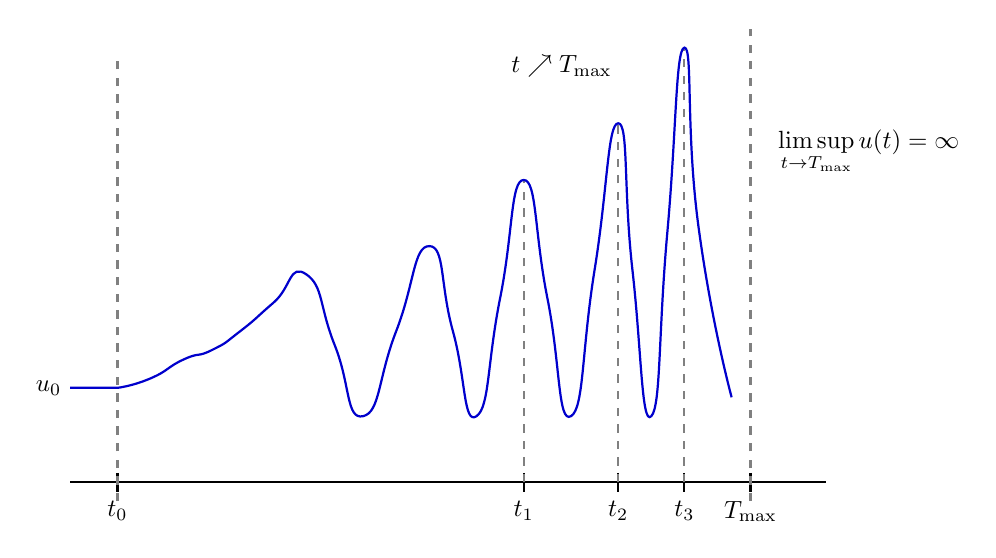
\begin{tikzpicture}[scale=1.2, every node/.style={scale=0.9}]
        % Eje horizontal (tiempo)
        \draw[thick] (0, 0) -- (8, 0);

        % Marcas y etiquetas en el eje X
        \draw[thick] (0.5, 0.1) -- (0.5, -0.1) node[below] {$t_0$};
        \draw[thick] (4.8, 0.1) -- (4.8, -0.1) node[below] {$t_1$};
        \draw[thick] (5.8, 0.1) -- (5.8, -0.1) node[below] {$t_2$};
        \draw[thick] (6.5, 0.1) -- (6.5, -0.1) node[below] {$t_3$};
        \draw[thick] (7.2, 0.1) -- (7.2, -0.1) node[below] {$T_{\max}$};

        % Líneas discontinuas verticales de los límites
        \draw[dashed, thick, gray] (0.5, -0.2) -- (0.5, 4.5);
        \draw[dashed, thick, gray] (7.2, -0.2) -- (7.2, 4.8);

        % Líneas discontinuas para los picos t1, t2, t3
        \draw[dashed, thick, gray] (4.8, 0) -- (4.8, 3.2);
        \draw[dashed, thick, gray] (5.8, 0) -- (5.8, 3.8);
        \draw[dashed, thick, gray] (6.5, 0) -- (6.5, 4.6);

        % Etiqueta del valor inicial u0
        \node[left] at (0, 1) {$u_0$};

        % Curva principal oscilante corregida mediante puntos intermedios (sin efecto globo)
        \draw[thick, blue!80!black] (0, 1) -- (0.5, 1)
            plot [smooth, tension=1.0] coordinates {
            (0.5, 1)
            (0.85, 1.1)
            (1.2, 1.3)
            (1.5, 1.4)
            (1.8, 1.6)
            (2.15, 1.9)
            (2.5, 2.2)
            (2.8, 1.45)
            (3.1, 0.7)
            (3.45, 1.6)
            (3.8, 2.5)
            (4.05, 1.6)
            (4.3, 0.7)
            (4.55, 1.95)
            (4.8, 3.2)
            (5.05, 1.95)
            (5.3, 0.7)
            (5.55, 2.25)
            (5.8, 3.8)
            (5.95, 2.25)
            (6.15, 0.7)
            (6.32, 2.65)
            (6.5, 4.6)
            (6.65, 2.7)
            (7.0, 0.9)
            };

        % Textos y límites
        \node at (5.2, 4.4) {$t \nearrow T_{\max}$};

        % El límite superior
        \node[right] at (7.4, 3.5) {$\displaystyle \limsup_{t \to T_{\max}} u(t) = \infty$};

    \end{tikzpicture}
    \end{center}

\end{observación}

Probemos ahora el teorema.

\begin{proof}
    Como hemos visto, tenemos 2 posibles casos.\\

    En el \textbf{primer caso}, si $I = J$, entonces la solución maximal está globalmente definida en todo el intervalo $J$, y por el Teorema de unicidad global, es la única solución de $(P)$ en $J$.\\

    Veamos ahora el \textbf{segundo caso}, que es más interesante, a priori tenemos dos posibilidades:
    \[
        \begin{cases}
            I = [t_0, T_{\text{max}}], \text{ con } T_{\text{max}} < t_0 + T \\
            \boxed{I = [t_0, T_{\text{max}}), \text{ con } T_{\text{max}} \leq t_0 + T}
        \end{cases}
    \]

    Probemos que la primera posibilidad es imposible, y después probemos la segunda
    \begin{enumerate}
        \item Supongamos que $I = [t_0, T_{\text{max}}]$, con $T_{\text{max}} < t_0 + T$.\\
        \item 
        Sabemos por RELLENAR, $\exists \delta > 0$ tal que el PVI tiene una única solución en el intervalo $[T_{\text{max}}, T_{\text{max}} + \delta]$, y por tanto podemos prolongar estrictamente la solución maximal $(I, u)$ a su derecha, lo cual es una contradicción de que $(I, u)$ sea maximal. Por lo tanto, la primera posibilidad es imposible.\\

        Si se quisiera extender la solución maximal a su derecha, se podría hacer definiendo la función:
        \[
            \widetilde{u}(t) =
            \begin{cases}
                u(t), & t \in [t_0, T_{\text{max}}] \\
                w(t), & t \in [T_{\text{max}}, T_{\text{max}} + \delta]
            \end{cases}
        \]
        Donde $w(t)$ es la solución del PVI:
        \[
            \begin{cases}
                w'(t) = f(t, w(t)) \\
                w(T_{\text{max}}) = u(T_{\text{max}})
            \end{cases}
        \]
        Y por el Teorema de unicidad global, $w(t)$ es la única solución de este PVI en el intervalo $[T_{\text{max}}, T_{\text{max}} + \delta]$, y además $\widetilde{u}(t)$ es continua y derivable en todo el intervalo $[t_0, T_{\text{max}} + \delta]$, por lo que $\widetilde{u}(t)$ es una prolongación estricta de la solución maximal $(I, u)$ a su derecha, lo cual es una contradicción.\\

        \item Ahora veamos el segundo caso, que es el más interesante.\\
        Supongamos que $I = [t_0, T_{\text{max}})$, con $T_{\text{max}} \leq t_0 + T$.\\

        Definamos además el conjunto:
        \[
            \Gamma = \{ u(t) : t \in I \} \text{ denominado órbita de } (I, u)
        \]
        
        Veremos más adelante la prueba de un lema que nos dice que si $\Gamma$ es no acotada, entonces la solución maximal $(I, u)$ explota en tiempo $T_{\text{max}}$.\\

        Ahora razonemos por reducción al absurdo. Supongamos que $\Gamma$ es acotada entonces $\overline{\Gamma}$ es compacto, y por tanto $J \times \overline{\Gamma}$ es compacto en $\mathbb{R} \times \mathbb{R}^N$.\\

        Sea ahora:
        \[
            \| f \|_\infty = \max_{\| f(t, x) \| : (t, x) \in J \times \overline{\Gamma}}
        \]
        Y sea la sucesión:
        \[
            t_n = T_{\text{max}} - \frac{1}{n} \nearrow T_{\text{max}}
        \]
        Ahora como $\Gamma$ es acotada, la sucesión $\{ u(t_n) \}_{n \geq 1}$ es acotada, y por, al ser una sucesión acotada en un compacto, podemos aplicar el teorema de Bolzano-Weierstrass, y por tanto existe una subsucesión convergente:
        \[
            \exists \mu(t_{n_m}) \to u^* \in \mathbb{R}^N
        \]
        Y por lo tanto también se cumple que:
        \[
            t_{n_m} \to T_{\text{max}} \implies
            u(t_{n_m}) \to u^* \in \mathbb{R}^N
        \]
        Ahora podemos desarrollar:
        \[
            \| u(t_{n_m}) - u(t) \| =
            \| \int_t^{t_{n_m}} u'(s) ds \| =
            \| \int_t^{t_{n_m}} f(s, u(s)) ds \| \leq
            \int_t^{t_{n_m}} \| f(s, u(s)) \| ds \leq
            \| f \|_\infty | t_{n_m} - t |
        \]
        Y por lo tanto, tomando el límite cuando $m \to \infty$:
        \[
            \| u^* - u(t) \| = \| f \|_\infty | T_{\text{max}} - t | 
        \]
        Prolongando así:
        \[
            \boxed{\lim_{t \nearrow T_{\text{max}}} u(t) = u^* \in \mathbb{R}^N}
        \]
        Pero esto contradice que la solución maximal $(I, u)$ no es prolongable estrictamente a su derecha, ya que habríamos prolongado la solución un punto.\\

        Nótese además que la derivada está bien definida en $T_{\text{max}}$, ya que:
        \[
            u'(t) = f(t, u(t)) \to f(T_{\text{max}}, u^*) \in \mathbb{R}^N
        \]

        Por tanto sabemos que $\Gamma$ es no acotada, pero falta ver que el punto de explosión es $T_{\text{max}}$.\\

        Sea una sucesión $t_n \in I$ tal que $\| u(t_n) \| \geq n$, como $t_n$ es acotada en un compacto hay una subsucesión convergente $t_{n_m} \to t^* \in [t_0, T_{\text{max}}]$, dónde:
        \[
            \| u(t_{n_m}) \| \geq n_m \to +\infty \implies
            \lim_{m \to \infty} \| u(t_{n_m}) \| = +\infty
        \]

        Pero ahora debemos probar que $t^* = T_{\text{max}}$, para que así se cumpla que:
        \[
            \varlimsup_{t \nearrow T_{\text{max}}} \| u(t) \| = +\infty
        \]
        
        Y así concluir que la solución maximal $(I, u)$ explota en tiempo $T_{\text{max}}$.\\
        RELLENAR ESTA PARTE
    \end{enumerate}
\end{proof}


\begin{teorema}[Segundo teorema fundamental de la teoría de Cauchy-Lipschitz]
    Sean $J = [t_0, +\infty)$, $f \in C(J \times \mathbb{R}^N, \mathbb{R}^N)$ una función localmente Lipschitziana respecto a $u \in \mathbb{R}^N$, uniformemente en subintervalos compactos de $J$, y sea $(I, u)$ la solución maximal del PVI:
    \[
        (P) =
        \begin{cases}
            u'(t) = f(t, u(t)) \\
            u(t_0) = u_0
        \end{cases}
    \]
    Entonces $I = [t_0, T_{\text{max}})$, con $T_{\text{max}} \in (t_0, +\infty]$, y en tal caso:
    \[
        \varlimsup_{t \nearrow T_{\text{max}}} \| u(t) \| = +\infty \quad \text{(si } T_{\text{max}} < +\infty \text{)}
    \]    
\end{teorema}

\begin{proof}
    Si $T_{\text{max}} = +\infty$, entonces $I = J = [t_0, +\infty)$, y la solución maximal está globalmente definida en todo el intervalo $J$. En este caso no hay explosión en tiempo finito.
    
    Supongamos que $I \subsetneq J$, es decir, $T_{\text{max}} < +\infty$. En principio, el intervalo maximal $I$ podría tener dos formas:
    \[
        \begin{cases}
            I = [t_0, T_{\text{max}}], \text{ con } T_{\text{max}} < +\infty \\
            I = [t_0, T_{\text{max}}), \text{ con } T_{\text{max}} < +\infty
        \end{cases}
    \]
    Pero el primer caso es imposible. Si $I = [t_0, T_{\text{max}}]$, el valor $u(T_{\text{max}}) \in \mathbb{R}^N$ estaría bien definido. Como $f$ satisface las hipótesis del teorema de existencia y unicidad local (Picard-Lindelöf), podríamos considerar un nuevo PVI tomando como instante inicial $T_{\text{max}}$:
    \[
        \begin{cases}
            w'(t) = f(t, w(t)) \\
            w(T_{\text{max}}) = u(T_{\text{max}})
        \end{cases}
    \]
    Esto nos garantizaría la existencia de una solución local $w$ definida en un intervalo $[T_{\text{max}}, T_{\text{max}} + \delta)$ con $\delta > 0$. Concatenando $u$ con $w$, obtendríamos una solución al problema original definida en $[t_0, T_{\text{max}} + \delta)$, lo cual contradice directamente la maximalidad del intervalo $I$. Por lo tanto, el intervalo debe ser necesariamente abierto por la derecha: $I = [t_0, T_{\text{max}})$.

    Tenemos que comprobar ahora que la solución $u(t)$ explota al acercarse a $T_{\text{max}}$, es decir, que la órbita:
    \[
        \Gamma = \{ u(t) : t \in [t_0, T_{\text{max}}) \} \text{ es no acotada}
    \]
    Supongamos por reducción al absurdo que $\Gamma$ es acotada. Entonces, su clausura $\overline{\Gamma}$ es un conjunto cerrado y acotado en $\mathbb{R}^N$, y por el Teorema de Heine-Borel, es compacto. 
    Definimos el cilindro compacto $K = [t_0, T_{\text{max}}] \times \overline{\Gamma} \subset \mathbb{R} \times \mathbb{R}^N$.
    
    Como $f$ es continua en $K$, alcanza un máximo por el teorema de Weierstrass. Podemos acotar su norma:
    \[
        \| f \|_\infty = \max_{(t, x) \in K} \| f(t, x) \| < +\infty
    \]
    Tomemos una sucesión de tiempos $t_n = T_{\text{max}} - \frac{1}{n}$ de manera que $t_n \nearrow T_{\text{max}}$. La sucesión de puntos correspondientes $\{u(t_n)\}_{n \geq 1} \subset \Gamma$ es acotada por hipótesis. Por el teorema de Bolzano-Weierstrass, existe una subsucesión convergente:
    \[
        \exists u(t_{n_m}) \xrightarrow[m \to \infty]{} u^* \in \mathbb{R}^N
    \]
    
    Por el Teorema Fundamental del Cálculo, para cualquier $t \in I$ y para nuestro $t_{n_m}$, se cumple que:
    \[
        u(t_{n_m}) - u(t) = \int_t^{t_{n_m}} u'(s) \, ds = \int_t^{t_{n_m}} f(s, u(s)) \, ds
    \]
    Tomando normas e introduciendo el valor absoluto en los límites de integración para asegurar que el intervalo es positivo, acotamos usando el supremo de $f$:
    \[
        \| u(t_{n_m}) - u(t) \| \leq \left| \int_t^{t_{n_m}} \| f(s, u(s)) \| \, ds \right| \leq \| f \|_\infty | t_{n_m} - t |
    \]
    Fijando $t$ y tomando el límite cuando $m \to \infty$ en la desigualdad, dado que $t_{n_m} \to T_{\text{max}}$ y $u(t_{n_m}) \to u^*$, obtenemos:
    \[
        \| u^* - u(t) \| \leq \| f \|_\infty | T_{\text{max}} - t |, \quad \forall t \in I
    \]
    Si ahora tomamos el límite cuando $t \nearrow T_{\text{max}}$, la parte derecha de la desigualdad tiende a $0$, lo que implica que:
    \[
        \lim_{t \nearrow T_{\text{max}}} u(t) = u^* \in \mathbb{R}^N
    \]
    Como el límite de $u(t)$ existe y es finito, podemos definir $u(T_{\text{max}}) = u^*$. Esto extiende la solución de forma continua al intervalo cerrado $[t_0, T_{\text{max}}]$, lo cual ya probamos en la primera parte que es imposible porque contradice la maximalidad de la solución.
    
    Esta contradicción proviene de suponer que $\Gamma$ es acotada. Por lo tanto, la órbita debe ser no acotada, concluyendo la demostración:
    \[
        \varlimsup_{t \nearrow T_{\text{max}}} \| u(t) \| = +\infty
    \]
\end{proof}

\[
    n \geq 1, \quad t_n \in T = [t_0, T_{\text{max}}), \quad \| u(t_n) \| \geq n
\]
\[
    \lim_{n \to \infty} \| u(t_n) \| = +\infty, \quad \{t_n\}_{n \geq 1} \text{ es acotada} 
\]
por Bolzano-Weierstrass, $\exists t_{n_m} \to t^* \in [t_0, T_{\text{max}}]$.
\[
    \begin{cases}
        t^* < T_{\text{max}} \\
        t^* = T_{\text{max}}
    \end{cases}
\]
\[
    \| u(t_{n_m}) \| \xrightarrow[m \to \infty]{} \| u(t^*) \| 
\]
\[
    \lim_{m \to \infty} \| u(t_{n_m}) \| = \| u(t^*) \| \quad \text{ contradicción}
\]
\[
    t^* = T_{\text{max}}, \quad t_{n_m} \nearrow T_{\text{max}} = t^*
\]
\[
    \| u(t_{n_m}) \| \xrightarrow[m \to \infty]{} +\infty, \quad \limsup_{t \nearrow T_{\text{max}}} \| u(t) \| = +\infty
\]


\begin{teorema} [Tercer teorema fundamental de la teoría de Cauchy-Lipschitz]
    Sean $J = [t_0, +\infty)$, $\Omega \subsetneq \mathbb{R}^N$ un conjunto abierto, $f \in C(J \times \Omega, \mathbb{R}^N)$ una función localmente Lipschitziana respecto a $u \in \Omega$, uniformemente en subintervalos compactos de $J$, y sea $(I, u)$ la solución maximal del PVI:
    \[
        (P) =
        \begin{cases}
            u'(t) = f(t, u(t)) \\
            u(t_0) = u_0
        \end{cases}
    \]
    Entonces $I = [t_0, T_{\text{max}})$ para algún $T_{\text{max}} \in (t_0, +\infty]$. Además, cuando $T_{\text{max}} < +\infty$, se cumple al menos una de las siguientes alternativas:
    \begin{enumerate}
        \item Explosión en tiempo $T_{\text{max}}$:
        \[
            \varlimsup_{t \nearrow T_{\text{max}}} \| u(t) \| = +\infty
        \]
        \item $\exists t\{t_n\}_{n \geq 1} \subset I$ y $u_\omega \in \partial \Omega$ tal que:
        \[
            \lim_{n \to \infty} u(t_n) = u_\omega \in \partial \Omega
        \]
        (la solución se acerca a la frontera del conjunto abierto $\Omega$)
    \end{enumerate}
\end{teorema}

\begin{proof}
    Si $I = J = [t_0, +\infty)$, entonces la solución maximal está globalmente definida en todo el intervalo $J$. En este caso no hay explosión en tiempo finito ni acercamiento a la frontera de $\Omega$.
    Supongamos que $I \subsetneq J$, entonces $I = [t_0, T_{\text{max}})$ o $I = [t_0, T_{\text{max}}]$ para algún $T_{\text{max}} < +\infty$. Como ya probamos en el teorema anterior, el caso $I = [t_0, T_{\text{max}}]$ es imposible, por lo que necesariamente $I = [t_0, T_{\text{max}})$.
    \[
        \Gamma = \{ u(t) : t \in [t_0, T_{\text{max}}) \}
    \]
    entonces
    \[
        \begin{cases}
            \Gamma \text{ es no acotada} \implies \varlimsup_{t \nearrow T_{\text{max}}} \| u(t) \| = +\infty \\
            \Gamma \text{ es acotada} \implies \overline{\Gamma} \subset \overline{\Omega}
        \end{cases}
    \]
    \begin{itemize}
        \item O bien $\overline{\Gamma} \subset \Omega$ \item O bien $\overline{\Gamma} \cap \partial \Omega \neq \emptyset$
    \end{itemize}

    Veamos el primer caso. Supongamos que $\overline{\Gamma} \subset \Omega$. Entonces,
    \[
        \| f \|_\infty = \max_{(t, x) \in [t_0, T_{\text{max}}] \times \overline{\Gamma}} \| f(t, x) \| < +\infty
    \]
    es importante que $\overline{\Gamma} \subset \Omega$ ya que $f$ puede no estar definida en $\partial \Omega$.\\
    Tomamos una sucesión de tiempos $t_n = T_{\text{max}} - \frac{1}{n}$ de manera que $t_n \nearrow T_{\text{max}}$. La sucesión de puntos correspondientes $\{u(t_n)\}_{n \geq 1} \subset \Gamma$ es acotada (porque $\overline{\Gamma}$ es compacto). Por el teorema de Bolzano-Weierstrass, existe una subsucesión convergente:
    \[
        \exists u(t_{n_m}) \xrightarrow[m \to \infty]{} u^* \in \overline{\Gamma} \subset \Omega
    \]
    \[
        \| u(t_{n_m}) - u(t) \| = \left\| \int_t^{t_{n_m}} \underbrace{f(s, u(s))}_{u'(s)} ds \right\| \leq \int_t^{t_{n_m}} \| f(s, u(s)) \| ds \leq \| f \|_\infty | t_{n_m} - t |
    \]
    En el límite cuando $m \to \infty$:
    \[
        \| u^* - u(t) \| \leq \| f \|_\infty | T_{\text{max}} - t |, \quad \forall t \in I
    \]
    Tomando el límite cuando $t \nearrow T_{\text{max}}$, obtenemos:
    \[
        \lim_{t \nearrow T_{\text{max}}} u(t) = u^* \in \Omega
    \]
    Esto contradice que la solución maximal $(I, u)$ no es prolongable estrictamente a su derecha, ya que habríamos prolongado la solución un punto. Por lo tanto, el primer caso es imposible.\\
    Por lo tanto, necesariamente se cumple que $\overline{\Gamma} \cap \partial \Omega \neq \emptyset$, es decir, la solución se acerca a la frontera del conjunto abierto $\Omega$.
    \[
        \exists u_\omega \in \partial \Omega \cap \overline{\Gamma} 
    \]
    \[
        u(t_n) \in \Gamma, \quad t_n \in I = [t_0, T_{\text{max}}), \quad u(t_n) \to u_\omega \in \partial \Omega
    \]
    \[
        \{t_n\}_{n \geq 1} \text{ acotada }
    \]
    por el teorema de Bolzano-Weierstrass, $\exists t_{n_m} \to t^* \in [t_0, T_{\text{max}}]$.\\
    Veamos que $t^* = T_{\text{max}}$. Supongamos que $t^* < T_{\text{max}}$. Entonces, por continuidad de $u(t)$ en $[t_0, T_{\text{max}})$:
    \[
        u(t_{n_m}) \to u(t^*) \in \Omega
    \]
    Pero esto contradice que $u(t_{n_m}) \to u_\omega \in \partial \Omega$. Por lo tanto, necesariamente $t^* = T_{\text{max}}$, y así se cumple que:
    \[
        u(t_n) \to u_\omega \in \partial \Omega, \quad t_n \nearrow T_{\text{max}}
    \]

\end{proof}


\ejemplo{
    \begin{center}
    \begin{tikzpicture}[thick, >=stealth]

    % Fronteras superior e inferior
    \draw (-4, 1.5) -- (4, 1.5);
    \draw (-4, -1.5) -- (4, -1.5);

    % Relleno de lineas (hatching) para representar el exterior del dominio
    % Requiere: \usetikzlibrary{patterns}
    \fill[pattern=north east lines, pattern color=black] (-4, 1.5) rectangle (4, 2.5);
    \fill[pattern=north east lines, pattern color=black] (-4, -2.5) rectangle (4, -1.5);

    % Etiqueta del dominio Omega a la izquierda
    \draw[->, thick] (-5.5, 0) -- (-4.5, 0);
    \node[anchor=east] at (-5.6, 0) {\Large $\Omega$};

    % Punto central u_0
    \coordinate (U0) at (0, 0);
    \fill (U0) circle (2pt);
    \node[anchor=north, yshift=-3pt] at (U0) {$u_0$};

    % Espiral centrada en u_0 (achatada para ajustarse a la franja)
    % Da ~4 vueltas expandiéndose horizontalmente hasta ~3.2 y verticalmente hasta ~1.3
    \draw[domain=0:1440, samples=350, smooth] 
        plot ({0.0022 * \x * cos(\x)}, {0.0009 * \x * sin(\x)});

    % Línea punteada azul hacia la frontera superior
    \draw[cyan, densely dashed, line width=1.5pt] (U0) -- (0, 1.5);

    % Línea discontinua roja hacia la derecha cortando las órbitas
    \draw[red, dashed, line width=1.5pt] (U0) -- (3.5, 0);

    % Puntos de intersección superiores (con el radio cyan: theta = 90 + 360*k)
    % y = 0.0009 * theta -> theta = 90, 450, 810, 1170
    \foreach \ang in {90, 450, 810, 1170} {
        \fill[cyan!80!blue] (0, {0.0009 * \ang}) circle (2.2pt);
    }

    % Puntos de intersección a la derecha (con el radio rojo: theta = 360*k)
    % x = 0.0022 * theta -> theta = 360, 720, 1080, 1440
    \foreach \ang in {360, 720, 1080, 1440} {
        \fill[red] ({0.0022 * \ang}, 0) circle (2.2pt);
    }

    % Anotaciones de las sucesiones a la derecha
    \node[anchor=west] at (4.5, 0.6) {$u(s_n), \, n \ge 1 \quad \|u(s_n)\| \xrightarrow{n \to \infty} +\infty$};
    \node[anchor=west] at (4.5, -0.6) {$u(t_n), \, n \ge 1 \quad u(t_n) \xrightarrow{n \to \infty} u_\omega \in \Omega$};

    \end{tikzpicture}
    \end{center}    
}

\begin{teorema}
    Sean $J = [t_0, t_0 + T]$, $\Omega = B_R(q)$, $f \in C(J \times \overline{\Omega}, \mathbb{R}^N)$ una función globalmente Lipschitziana respecto a $u \in \overline{\Omega}$, uniformemente en $t \in J$. Entonces para cada $u_0 \in \Omega$, el PVI:
    \[
        (P) =
        \begin{cases}
            u'(t) = f(t, u(t)) \\
            u(t_0) = u_0
        \end{cases}
    \]
    tiene una única solución $(I_{\text{max}}, u_{\text{max}})$ maximal. Además, o bien $I_{\text{max}} = J$, o bien $I_{\text{max}} = [t_0, T_{\text{max}}]$, con $T_{\text{max}} \leq t_0 + T$, y cuando $T_{\text{max}} < t_0 + T$, se cumple que:
    \[
        u_{\text{max}}(T_{\text{max}}) \in \partial \Omega
    \]
\end{teorema}

\begin{proof}
    Sea $\Sigma$ el conjunto de soluciones del PVI $(P)$, entonces $\Sigma \neq \emptyset$ por el teorema de Cauchy-Lipschitz local.
    \[
        u_I(t) \in \overline{\Omega}, \quad \forall t \in I
    \]
    \[
        u_I'(t) = f(t, u_I(t)) \in 
    \]
    \[
        I_{\text{max}} = \bigcup_{(I, u_I) \in \Sigma} I
    \]
    \[
        u_{\text{max}}(t) = u_I(t), \quad t \in I
    \]
\end{proof}
